%% bare_jrnl.tex
%% V1.3
%% 2007/01/11
%% by Michael Shell
%% see http://www.michaelshell.org/
%% for current contact information.
%%
%% This is a skeleton file demonstrating the use of IEEEtran.cls
%% (requires IEEEtran.cls version 1.7 or later) with an IEEE journal paper.
%%
%% Support sites:
%% http://www.michaelshell.org/tex/ieeetran/
%% http://www.ctan.org/tex-archive/macros/latex/contrib/IEEEtran/
%% and
%% http://www.ieee.org/



% *** Authors should verify (and, if needed, correct) their LaTeX system  ***
% *** with the testflow diagnostic prior to trusting their LaTeX platform ***
% *** with production work. IEEE's font choices can trigger bugs that do  ***
% *** not appear when using other class files.                            ***
% The testflow support page is at:
% http://www.michaelshell.org/tex/testflow/


%%*************************************************************************
%% Legal Notice:
%% This code is offered as-is without any warranty either expressed or
%% implied; without even the implied warranty of MERCHANTABILITY or
%% FITNESS FOR A PARTICULAR PURPOSE! 
%% User assumes all risk.
%% In no event shall IEEE or any contributor to this code be liable for
%% any damages or losses, including, but not limited to, incidental,
%% consequential, or any other damages, resulting from the use or misuse
%% of any information contained here.
%%
%% All comments are the opinions of their respective authors and are not
%% necessarily endorsed by the IEEE.
%%
%% This work is distributed under the LaTeX Project Public License (LPPL)
%% ( http://www.latex-project.org/ ) version 1.3, and may be freely used,
%% distributed and modified. A copy of the LPPL, version 1.3, is included
%% in the base LaTeX documentation of all distributions of LaTeX released
%% 2003/12/01 or later.
%% Retain all contribution notices and credits.
%% ** Modified files should be clearly indicated as such, including  **
%% ** renaming them and changing author support contact information. **
%%
%% File list of work: IEEEtran.cls, IEEEtran_HOWTO.pdf, bare_adv.tex,
%%                    bare_conf.tex, bare_jrnl.tex, bare_jrnl_compsoc.tex
%%*************************************************************************

% Note that the a4paper option is mainly intended so that authors in
% countries using A4 can easily print to A4 and see how their papers will
% look in print - the typesetting of the document will not typically be
% affected with changes in paper size (but the bottom and side margins will).
% Use the testflow package mentioned above to verify correct handling of
% both paper sizes by the user's LaTeX system.
%
% Also note that the "draftcls" or "draftclsnofoot", not "draft", option
% should be used if it is desired that the figures are to be displayed in
% draft mode.
%
\documentclass[journal]{IEEEtran}
%
% If IEEEtran.cls has not been installed into the LaTeX system files,
% manually specify the path to it like:
% \documentclass[journal]{../sty/IEEEtran}





% Some very useful LaTeX packages include:
% (uncomment the ones you want to load)


% *** MISC UTILITY PACKAGES ***
%
%\usepackage{ifpdf}
% Heiko Oberdiek's ifpdf.sty is very useful if you need conditional
% compilation based on whether the output is pdf or dvi.
% usage:
% \ifpdf
%   % pdf code
% \else
%   % dvi code
% \fi
% The latest version of ifpdf.sty can be obtained from:
% http://www.ctan.org/tex-archive/macros/latex/contrib/oberdiek/
% Also, note that IEEEtran.cls V1.7 and later provides a builtin
% \ifCLASSINFOpdf conditional that works the same way.
% When switching from latex to pdflatex and vice-versa, the compiler may
% have to be run twice to clear warning/error messages.






% *** CITATION PACKAGES ***
%
%\usepackage{cite}
% cite.sty was written by Donald Arseneau
% V1.6 and later of IEEEtran pre-defines the format of the cite.sty package
% \cite{} output to follow that of IEEE. Loading the cite package will
% result in citation numbers being automatically sorted and properly
% "compressed/ranged". e.g., [1], [9], [2], [7], [5], [6] without using
% cite.sty will become [1], [2], [5]--[7], [9] using cite.sty. cite.sty's
% \cite will automatically add leading space, if needed. Use cite.sty's
% noadjust option (cite.sty V3.8 and later) if you want to turn this off.
% cite.sty is already installed on most LaTeX systems. Be sure and use
% version 4.0 (2003-05-27) and later if using hyperref.sty. cite.sty does
% not currently provide for hyperlinked citations.
% The latest version can be obtained at:
% http://www.ctan.org/tex-archive/macros/latex/contrib/cite/
% The documentation is contained in the cite.sty file itself.






% *** GRAPHICS RELATED PACKAGES ***
%
\ifCLASSINFOpdf
  % \usepackage[pdftex]{graphicx}
  % declare the path(s) where your graphic files are
  % \graphicspath{{../pdf/}{../jpeg/}}
  % and their extensions so you won't have to specify these with
  % every instance of \includegraphics
  % \DeclareGraphicsExtensions{.pdf,.jpeg,.png}
\else
  % or other class option (dvipsone, dvipdf, if not using dvips). graphicx
  % will default to the driver specified in the system graphics.cfg if no
  % driver is specified.
  % \usepackage[dvips]{graphicx}
  % declare the path(s) where your graphic files are
  % \graphicspath{{../eps/}}
  % and their extensions so you won't have to specify these with
  % every instance of \includegraphics
  % \DeclareGraphicsExtensions{.eps}
\fi
% graphicx was written by David Carlisle and Sebastian Rahtz. It is
% required if you want graphics, photos, etc. graphicx.sty is already
% installed on most LaTeX systems. The latest version and documentation can
% be obtained at: 
% http://www.ctan.org/tex-archive/macros/latex/required/graphics/
% Another good source of documentation is "Using Imported Graphics in
% LaTeX2e" by Keith Reckdahl which can be found as epslatex.ps or
% epslatex.pdf at: http://www.ctan.org/tex-archive/info/
%
% latex, and pdflatex in dvi mode, support graphics in encapsulated
% postscript (.eps) format. pdflatex in pdf mode supports graphics
% in .pdf, .jpeg, .png and .mps (metapost) formats. Users should ensure
% that all non-photo figures use a vector format (.eps, .pdf, .mps) and
% not a bitmapped formats (.jpeg, .png). IEEE frowns on bitmapped formats
% which can result in "jaggedy"/blurry rendering of lines and letters as
% well as large increases in file sizes.
%
% You can find documentation about the pdfTeX application at:
% http://www.tug.org/applications/pdftex





% *** MATH PACKAGES ***
%
%\usepackage[cmex10]{amsmath}
% A popular package from the American Mathematical Society that provides
% many useful and powerful commands for dealing with mathematics. If using
% it, be sure to load this package with the cmex10 option to ensure that
% only type 1 fonts will utilized at all point sizes. Without this option,
% it is possible that some math symbols, particularly those within
% footnotes, will be rendered in bitmap form which will result in a
% document that can not be IEEE Xplore compliant!
%
% Also, note that the amsmath package sets \interdisplaylinepenalty to 10000
% thus preventing page breaks from occurring within multiline equations. Use:
%\interdisplaylinepenalty=2500
% after loading amsmath to restore such page breaks as IEEEtran.cls normally
% does. amsmath.sty is already installed on most LaTeX systems. The latest
% version and documentation can be obtained at:
% http://www.ctan.org/tex-archive/macros/latex/required/amslatex/math/





% *** SPECIALIZED LIST PACKAGES ***
%
%\usepackage{algorithmic}
% algorithmic.sty was written by Peter Williams and Rogerio Brito.
% This package provides an algorithmic environment fo describing algorithms.
% You can use the algorithmic environment in-text or within a figure
% environment to provide for a floating algorithm. Do NOT use the algorithm
% floating environment provided by algorithm.sty (by the same authors) or
% algorithm2e.sty (by Christophe Fiorio) as IEEE does not use dedicated
% algorithm float types and packages that provide these will not provide
% correct IEEE style captions. The latest version and documentation of
% algorithmic.sty can be obtained at:
% http://www.ctan.org/tex-archive/macros/latex/contrib/algorithms/
% There is also a support site at:
% http://algorithms.berlios.de/index.html
% Also of interest may be the (relatively newer and more customizable)
% algorithmicx.sty package by Szasz Janos:
% http://www.ctan.org/tex-archive/macros/latex/contrib/algorithmicx/




% *** ALIGNMENT PACKAGES ***
%
%\usepackage{array}
% Frank Mittelbach's and David Carlisle's array.sty patches and improves
% the standard LaTeX2e array and tabular environments to provide better
% appearance and additional user controls. As the default LaTeX2e table
% generation code is lacking to the point of almost being broken with
% respect to the quality of the end results, all users are strongly
% advised to use an enhanced (at the very least that provided by array.sty)
% set of table tools. array.sty is already installed on most systems. The
% latest version and documentation can be obtained at:
% http://www.ctan.org/tex-archive/macros/latex/required/tools/


%\usepackage{mdwmath}
%\usepackage{mdwtab}
% Also highly recommended is Mark Wooding's extremely powerful MDW tools,
% especially mdwmath.sty and mdwtab.sty which are used to format equations
% and tables, respectively. The MDWtools set is already installed on most
% LaTeX systems. The lastest version and documentation is available at:
% http://www.ctan.org/tex-archive/macros/latex/contrib/mdwtools/


% IEEEtran contains the IEEEeqnarray family of commands that can be used to
% generate multiline equations as well as matrices, tables, etc., of high
% quality.


%\usepackage{eqparbox}
% Also of notable interest is Scott Pakin's eqparbox package for creating
% (automatically sized) equal width boxes - aka "natural width parboxes".
% Available at:
% http://www.ctan.org/tex-archive/macros/latex/contrib/eqparbox/





% *** SUBFIGURE PACKAGES ***
%\usepackage[tight,footnotesize]{subfigure}
% subfigure.sty was written by Steven Douglas Cochran. This package makes it
% easy to put subfigures in your figures. e.g., "Figure 1a and 1b". For IEEE
% work, it is a good idea to load it with the tight package option to reduce
% the amount of white space around the subfigures. subfigure.sty is already
% installed on most LaTeX systems. The latest version and documentation can
% be obtained at:
% http://www.ctan.org/tex-archive/obsolete/macros/latex/contrib/subfigure/
% subfigure.sty has been superceeded by subfig.sty.



%\usepackage[caption=false]{caption}
%\usepackage[font=footnotesize]{subfig}
% subfig.sty, also written by Steven Douglas Cochran, is the modern
% replacement for subfigure.sty. However, subfig.sty requires and
% automatically loads Axel Sommerfeldt's caption.sty which will override
% IEEEtran.cls handling of captions and this will result in nonIEEE style
% figure/table captions. To prevent this problem, be sure and preload
% caption.sty with its "caption=false" package option. This is will preserve
% IEEEtran.cls handing of captions. Version 1.3 (2005/06/28) and later 
% (recommended due to many improvements over 1.2) of subfig.sty supports
% the caption=false option directly:
%\usepackage[caption=false,font=footnotesize]{subfig}
%
% The latest version and documentation can be obtained at:
% http://www.ctan.org/tex-archive/macros/latex/contrib/subfig/
% The latest version and documentation of caption.sty can be obtained at:
% http://www.ctan.org/tex-archive/macros/latex/contrib/caption/




% *** FLOAT PACKAGES ***
%
%\usepackage{fixltx2e}
% fixltx2e, the successor to the earlier fix2col.sty, was written by
% Frank Mittelbach and David Carlisle. This package corrects a few problems
% in the LaTeX2e kernel, the most notable of which is that in current
% LaTeX2e releases, the ordering of single and double column floats is not
% guaranteed to be preserved. Thus, an unpatched LaTeX2e can allow a
% single column figure to be placed prior to an earlier double column
% figure. The latest version and documentation can be found at:
% http://www.ctan.org/tex-archive/macros/latex/base/



%\usepackage{stfloats}
% stfloats.sty was written by Sigitas Tolusis. This package gives LaTeX2e
% the ability to do double column floats at the bottom of the page as well
% as the top. (e.g., "\begin{figure*}[!b]" is not normally possible in
% LaTeX2e). It also provides a command:
%\fnbelowfloat
% to enable the placement of footnotes below bottom floats (the standard
% LaTeX2e kernel puts them above bottom floats). This is an invasive package
% which rewrites many portions of the LaTeX2e float routines. It may not work
% with other packages that modify the LaTeX2e float routines. The latest
% version and documentation can be obtained at:
% http://www.ctan.org/tex-archive/macros/latex/contrib/sttools/
% Documentation is contained in the stfloats.sty comments as well as in the
% presfull.pdf file. Do not use the stfloats baselinefloat ability as IEEE
% does not allow \baselineskip to stretch. Authors submitting work to the
% IEEE should note that IEEE rarely uses double column equations and
% that authors should try to avoid such use. Do not be tempted to use the
% cuted.sty or midfloat.sty packages (also by Sigitas Tolusis) as IEEE does
% not format its papers in such ways.


%\ifCLASSOPTIONcaptionsoff
%  \usepackage[nomarkers]{endfloat}
% \let\MYoriglatexcaption\caption
% \renewcommand{\caption}[2][\relax]{\MYoriglatexcaption[#2]{#2}}
%\fi
% endfloat.sty was written by James Darrell McCauley and Jeff Goldberg.
% This package may be useful when used in conjunction with IEEEtran.cls'
% captionsoff option. Some IEEE journals/societies require that submissions
% have lists of figures/tables at the end of the paper and that
% figures/tables without any captions are placed on a page by themselves at
% the end of the document. If needed, the draftcls IEEEtran class option or
% \CLASSINPUTbaselinestretch interface can be used to increase the line
% spacing as well. Be sure and use the nomarkers option of endfloat to
% prevent endfloat from "marking" where the figures would have been placed
% in the text. The two hack lines of code above are a slight modification of
% that suggested by in the endfloat docs (section 8.3.1) to ensure that
% the full captions always appear in the list of figures/tables - even if
% the user used the short optional argument of \caption[]{}.
% IEEE papers do not typically make use of \caption[]'s optional argument,
% so this should not be an issue. A similar trick can be used to disable
% captions of packages such as subfig.sty that lack options to turn off
% the subcaptions:
% For subfig.sty:
% \let\MYorigsubfloat\subfloat
% \renewcommand{\subfloat}[2][\relax]{\MYorigsubfloat[]{#2}}
% For subfigure.sty:
% \let\MYorigsubfigure\subfigure
% \renewcommand{\subfigure}[2][\relax]{\MYorigsubfigure[]{#2}}
% However, the above trick will not work if both optional arguments of
% the \subfloat/subfig command are used. Furthermore, there needs to be a
% description of each subfigure *somewhere* and endfloat does not add
% subfigure captions to its list of figures. Thus, the best approach is to
% avoid the use of subfigure captions (many IEEE journals avoid them anyway)
% and instead reference/explain all the subfigures within the main caption.
% The latest version of endfloat.sty and its documentation can obtained at:
% http://www.ctan.org/tex-archive/macros/latex/contrib/endfloat/
%
% The IEEEtran \ifCLASSOPTIONcaptionsoff conditional can also be used
% later in the document, say, to conditionally put the References on a 
% page by themselves.





% *** PDF, URL AND HYPERLINK PACKAGES ***
%
%\usepackage{url}
% url.sty was written by Donald Arseneau. It provides better support for
% handling and breaking URLs. url.sty is already installed on most LaTeX
% systems. The latest version can be obtained at:
% http://www.ctan.org/tex-archive/macros/latex/contrib/misc/
% Read the url.sty source comments for usage information. Basically,
% \url{my_url_here}.





% *** Do not adjust lengths that control margins, column widths, etc. ***
% *** Do not use packages that alter fonts (such as pslatex).         ***
% There should be no need to do such things with IEEEtran.cls V1.6 and later.
% (Unless specifically asked to do so by the journal or conference you plan
% to submit to, of course. )


% correct bad hyphenation here
\hyphenation{op-tical net-works semi-conduc-tor ordering algorithms}


\usepackage{bm,subfigure,graphicx,url,times,multirow,amsmath,amssymb,algorithm,xspace,epsfig,todonotes,array,caption,color,todonotes}
\usepackage{algorithm, mathtools}
\usepackage[noend]{algpseudocode}
\usepackage[bookmarks=false]{hyperref}
\hyphenation{op-tical net-works semi-conduc-tor IEEEtran instead}

\newcommand{\degree}{^{\circ}}
\newcommand{\set}[1]{\left\{#1\right\}}
\newcommand{\setb}[2]{\set{#1 \ : \ #2}}
\newcommand{\argmax}{\operatorname*{arg\,max}}

\newcommand{\twoIndent}{\hskip\algorithmicindent\hskip\algorithmicindent}
\newcommand{\threeIndent}{\hskip\algorithmicindent\hskip\algorithmicindent\hskip\algorithmicindent}

\begin{document}
%
% paper title
% can use linebreaks \\ within to get better formatting as desired


\title{\ \\ \LARGE\bf Multi-Objective Monte Carlo Tree Search for Real-Time Games \thanks{Diego~Perez, Spyridon~Samothrakis, Simon~M.~Lucas (School of Computer Science and Electronic Engineering, University of Essex, Colchester CO4 3SQ, UK; email: {\tt \{dperez,ssamot,sml\}@essex.ac.uk}); \newline
Sanaz~Mostaghim (Department of Knowledge and Language Engineering, Otto-von-Guericke-Universität Magdeburg, Magdeburg, Germany; email: {\tt sanaz.mostaghim@ovgu.de})}}

%
%
% author names and IEEE memberships
% note positions of commas and nonbreaking spaces ( ~ ) LaTeX will not break
% a structure at a ~ so this keeps an author's name from being broken across
% two lines.
% use \thanks{} to gain access to the first footnote area
% a separate \thanks must be used for each paragraph as LaTeX2e's \thanks
% was not built to handle multiple paragraphs
%

\author{Diego Perez, {\it Student Member, IEEE}, Sanaz Mostaghim {Member, IEEE}, Spyridon Samothrakis, {\it Student Member, IEEE}, Simon M. Lucas, {\it Senior Member, IEEE}}

% note the % following the last \IEEEmembership and also \thanks - 
% these prevent an unwanted space from occurring between the last author name
% and the end of the author line. i.e., if you had this:
% 
% \author{....lastname \thanks{...} \thanks{...} }
%                     ^------------^------------^----Do not want these spaces!
%
% a space would be appended to the last name and could cause every name on that
% line to be shifted left slightly. This is one of those "LaTeX things". For
% instance, "\textbf{A} \textbf{B}" will typeset as "A B" not "AB". To get
% "AB" then you have to do: "\textbf{A}\textbf{B}"
% \thanks is no different in this regard, so shield the last } of each \thanks
% that ends a line with a % and do not let a space in before the next \thanks.
% Spaces after \IEEEmembership other than the last one are OK (and needed) as
% you are supposed to have spaces between the names. For what it is worth,
% this is a minor point as most people would not even notice if the said evil
% space somehow managed to creep in.



% The paper headers
\markboth{IEEE Transactions on Computational Intelligence and AI in Games}%
{Shell \MakeLowercase{\textit{et al.}}: Bare Demo of IEEEtran.cls for Journals}

% The only time the second header will appear is for the odd numbered pages
% after the title page when using the twoside option.
% 
% *** Note that you probably will NOT want to include the author's ***
% *** name in the headers of peer review papers.                   ***
% You can use \ifCLASSOPTIONpeerreview for conditional compilation here if
% you desire.




% If you want to put a publisher's ID mark on the page you can do it like
% this:
%\IEEEpubid{0000--0000/00\$00.00~\copyright~2007 IEEE}
% Remember, if you use this you must call \IEEEpubidadjcol in the second
% column for its text to clear the IEEEpubid mark.



% use for special paper notices
%\IEEEspecialpapernotice{(Invited Paper)}




\maketitle

\begin{abstract}
Multi-objective optimization has been traditionally a matter of study in domains like engineering or finance, with little impact on games research. However, action-decision based on multi-objective evaluation may be beneficial in order to obtain a high quality level of play. This paper presents a Multi-objective Monte Carlo Tree Search algorithm for planning and control in real-time game domains, those where the time budget to decide the next move to make is close to 40ms. A comparison is made between the proposed algorithm, a single-objective version of Monte Carlo Tree Search and a rolling horizon implementation of Non-dominated Sorting Evolutionary Algorithm II (NSGA-II). Two different benchmarks are employed, Deep Sea Treasure and the Multi-Objective Physical Travelling Salesman Problem. Using the same heuristics on each game, the analysis is focused on how well the algorithms explore the search space. Results show that the algorithm proposed outperforms NSGA-II. Additionally, it is also shown that the algorithm is able to converge to different optimal solutions or the optimal Pareto front (if achieved during search).
\end{abstract}


% IEEEtran.cls defaults to using nonbold math in the Abstract.
% This preserves the distinction between vectors and scalars. However,
% if the journal you are submitting to favors bold math in the abstract,
% then you can use LaTeX's standard command \boldmath at the very start
% of the abstract to achieve this. Many IEEE journals frown on math
% in the abstract anyway.



% For peer review papers, you can put extra information on the cover
% page as needed:
% \ifCLASSOPTIONpeerreview
% \begin{center} \bfseries EDICS Category: 3-BBND \end{center}
% \fi
%
% For peerreview papers, this IEEEtran command inserts a page break and
% creates the second title. It will be ignored for other modes.
\IEEEpeerreviewmaketitle


%\IEEEoverridecommandlockouts
%
%\textwidth 178mm
%\textheight 239mm
%\oddsidemargin -7mm
%\evensidemargin -7mm
%\topmargin -6mm
%\columnsep 5mm


\section{Introduction} \label{sec:intro}

Multi-objective optimization has been a field of study in manufacturing, engineering~\cite{Marler2004} and finance~\cite{Coello2006}, while having little impact on games research. This paper shows that multi-objective optimization has much to offer in developing game strategies that allow for a fine-grained control of alternative policies. The application of such approaches to this field can provide interesting results, especially in games that are long or complex enough that long-term planning is not trivial, and achieving a good level of play requires balancing strategies.

At their most basic, many competitive games can be viewed as simply two or more opponents having the single objective of winning. Achieving victory is usually complex in interesting games, and successful approaches normally assign some form of value to a state, value being long term expected reward (i.e. expectation of victory). Due to a massive search space, heuristics are often used for this value function. An example is a chess heuristic that assigns different weights to each piece according to an estimated value.

Multi-objective approaches can be applied to scenarios where several factors must be taken into account to achieve victory. The algorithms can balance between different objectives, in order to provide a wide range of strategies well suited to the different stages of the game being played, or to face existing opponents. Application of such approaches could be real-time strategy games, where long term planning must be carried out in order to balance aspects such as attack units, defensive structures and resource gathering. This should allow allow smart balancing of heuristics. 

This paper proposes a multi-objective real-time algorithm version of Monte Carlo Tree Search (MCTS), a popular reinforcement learning approach that emerged in the last decade. The proposed algorithm is tested in two different games: a real-time version of the Deep Sea Treasure (DST; a classical multi-objective problem), and the Multi-Objective Physical Travelling Salesman Problem (MO-PTSP). The algorithm is also compared with another two approaches: a single-objective MCTS (that uses a weighted sum of features to value the state) and a rolling horizon Non-dominated Sorting Evolutionary Algorithm II (NSGA-II). This paper extends and formalizes our previous work described in~\cite{Perez2013a}.

Two main goals can be identified in this paper: first, the proposed algorithm must be applicable to real-time domains (those where the next move to make must be decided within a small time budget) and it should obtain better or at least the same performance than the other state-of-the-art algorithms. It is important to highlight that all three algorithms tested employ the same heuristic functions to evaluate the features of a given game state. Thus, the focus of this research is set on how the algorithm explores the search space, instead of providing the best possible solution to each given problem. 

Secondly, the algorithm must be able to provide solutions across the multi-objective spectrum: by parametrizing the algorithm, it must be possible to prioritize one objective over the others and therefore converge to solutions according to these preferences. 

The paper is structured as follows. First, Sections~\ref{sec:mcts} and~\ref{sec:moo} provide the necessary background for MCTS and multi-objective optimization, respectively. The algorithm proposed in this research is described in detail in Section~\ref{sec:momcts}. Then, Section~\ref{sec:bench} defines the games used to test the algorithms, with the results discussed in Section~\ref{sec:exp}. Finally, some conclusions and possible extensions of this work are drawn in Section~\ref{sec:conc}.


\section{Monte Carlo Tree Search} \label{sec:mcts}

Monte Carlo Tree Search (MCTS) is a tree search algorithm that was originally applied to board games, gaining momentum and popularity in the game of Go. This game is played in a square grid board, with a size of $19 \times 19$ in the original game, and $9 \times 9$ in its reduced version. The game is played in turns, and the objective is to surround the opponent's stones by placing stones in any available position on the board. Due to the very large branching factor of Go, this game is considered the drosophila of Game AI, and MCTS players have reached professional level play in the reduced board size version~\cite{Lee2009}. After its success in Go, MCTS has been used extensively by many researchers in this and different domains. An extensive survey of MCTS methods, variations and applications, has been written by Browne et al.~\cite{Browne2012}. 

MCTS is considered to be an \textit{anytime} algorithm, as it is able to provide a valid next move to choose at any moment in time. This is true independently from how many iterations the algorithm is able to make (although, in general, more iterations usually produce better results). This differs from other algorithms (such as A* in single player games, and standard Min-Max for two player games) that normally provide the next play only after they have finished. This makes MCTS a suitable candidate for real-time domains, where the decision time budget is limited, affecting the number of iterations that can be performed.

MCTS is an algorithm that builds a tree in memory. Each node in the tree maintains statistics that indicate how often a move is played from a given state ($N(s,a)$), how many times each move is played from there ($N(s)$) and the average reward ($Q(s,a)$) obtained after applying move $a$ in state $s$. The tree is built iteratively by simulating actions in the game, making move choices based on statistics stored in the nodes. 

Each iteration of MCTS can be divided into several steps~\cite{Gelly2006}: \textit{Tree selection}, \textit{Expansion}, \textit{Monte Carlo simulation} and \textit{Back-propagation} (all summarized in Figure~\ref{fig:mcts}). When the algorithm starts, the tree is formed only by the root node, which holds the current state of the game. During the \textit{selection} step, the tree is navigated from the root until a maximum depth or the end of the game has been reached. 

\begin{figure} [!t]
	\begin{center}
	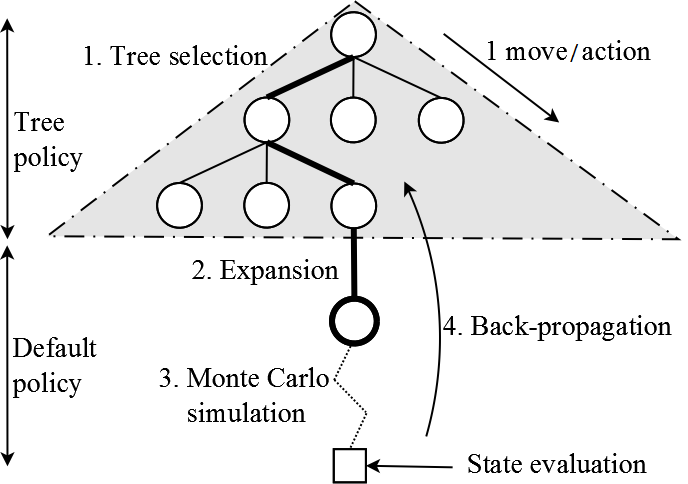
\includegraphics[scale=0.4,natwidth=708,natheight=484]{img/mcts.png}
	\caption{MCTS algorithm steps.}
	\label{fig:mcts}
	\end{center}
\end{figure}

In every one of these action decisions, MCTS balances between exploitation and exploration. In other words, it chooses between taking an action that leads to states with the best outcome found so far, and performing a move to go to less explored game states, respectively. In order to achieve this, MCTS uses Upper Confidence Bound (UCB1, see Equation~\ref{eq:ucb1}) as a \textit{Tree Policy}. 

\begin{equation}	\label{eq:ucb1}
a^* = \argmax_{a \in A(s)} \left\{Q(s,a) + C \sqrt{\frac{ \ln N(s) }{ N(s,a) }}\right\}
\end{equation}

The balance between exploration and exploitation can be tempered by modifying $C$. Higher values of $C$ give added weight to the second term of the UCB1 Equation~\ref{eq:ucb1}, giving preference to those actions that have been explored less, at the expense of taking actions with the highest average reward $Q(s,a)$. A commonly used value is $\sqrt{2}$, as it balances both facets of the search when the rewards are normalized between $0$ and $1$. It is worth noting that MCTS, when combined with UCB1, reaches asymptotically logarithmic regret on each node of the tree~\cite{coquelin2007bandit}. 

If, during the \textit{tree selection} phase, a node has fewer children than the available number of actions from a given position, a new node is added as a child of the current one (\textit{expansion} phase) and the \textit{simulation} step starts. At this point, MCTS executes a Monte Carlo simulation (or roll-out; \textit{default policy}) from the expanded node. This is performed by choosing random (either uniformly random, or biased) actions until the game end or a pre-defined depth is reached, where the state of the game is evaluated. 

Finally, during the \textit{back-propagation} step, the statistics $N(s)$, $N(s,a)$ and $Q(s,a)$ are updated for each node visited, using the reward obtained in the evaluation of the state. These steps are executed in a loop until a termination criteria is met (such as number of iterations).


MCTS has been employed extensively in real-time games. A clear example of this is the popular real-time game \textit{Ms. PacMan}. The objective of this game is to control Ms. PacMan to clear the maze by eating all pills, without being captured by the ghosts. An important feature of this game is that it is \textit{open-ended}, as an end game situation is, most of the time, far ahead in the future and can not be devised by the algorithm during its iterations. The consequence of this is that MCTS, in its vanilla form, it is not able to know if a given ply will lead to a win or a loss in the end game state. Robles et al.~\cite{Robles2009} solved this problem by including hand-coded heuristics that guided search towards more promising portions of the search space. This approach enabled the addition of heuristics knowledge to MCTS, as in~\cite{Samothrakis, Ikehata2010}.

MCTS has also been applied to single-player games, like SameGame~\cite{Matsumoto2010}, where the player's goal is to destroy contiguous tiles of the same colour, distributed in a rectangular grid. Another use of MCTS is in the popular puzzle Morpion Solitaire~\cite{Edelkamp2010}, a connection game where the goal is to link nodes of a graph with straight lines that must contain at least five vertices. Finally, the PTSP has also been addressed by MCTS, both in the single-objective~\cite{Perez2013, Powley2012} and the multi-objective versions~\cite{Powley2013}. These papers describe the entries that won both editions of the PTSP Competition.

It is worthwhile mentioning that in most cases found in the literature, MCTS techniques have been used with some kind of heuristic that guides the Monte Carlo simulations or the tree selection policy. In the algorithm proposed in this paper, simulations are purely random, as the objective is to compare the search abilities of the different algorithms. The intention is therefore to keep the heuristics to a minimum, and the existing pieces of domain knowledge are shared by all the algorithms presented (as in the case of the score function for MO-PTSP, described later).


\section{Multi-Objective Optimization} \label{sec:moo}

A multi-objective optimization problem (MOP) represents a scenario where two or more conflicting objective functions are to be optimized at the same time and is defined as: 
\begin{eqnarray}
optimize ~~~\{ f_1(\vec x), f_2(\vec x),\cdots , f_m(\vec x) \} 
\end{eqnarray}
subject to $\vec x \in \Omega$, involving $m (\geq 2)$ conflicting objective functions $f_i : \Re ^n \rightarrow \Re$. The \textit{decision vectors} 
$\vec x = (x_1, x_2, \cdots, x_n)^T$ belong to the feasible region $\Omega \subset \Re ^n$. We denote the image of the feasible region by $Z\subset \Re ^m$ and call it a feasible objective region. The
elements of $Z$ are called objective vectors and they consist of $m$ objective (function) values $\vec f(\vec x)= (f_1(\vec x), f_2(\vec x), \cdots, f_m(\vec x))$.
Therefore, each solution $\vec x$ provides $m$ different scores (or rewards, or fitness) that are meant to be optimized. Without loss of generality, it is assumed from now on that all objectives are to be maximized.

It is said that a solution $\vec x$ \textit{dominates} another solution $\vec y$ if and only if:
\begin{enumerate}
\item $f_i(\vec x)$ is not worse than $f_i(\vec y)$, $\forall i = 1, 2, \dots, m$.
\item For at least one objective $j$: $f_j(\vec x)$ is better than its analogous counterpart in $f_j(\vec y)$.
\end{enumerate}

When these two conditions apply, it is said that $\vec x \preceq \vec y$ ($\vec x$ dominates $\vec y$). The \textit{dominance} condition provides a partial ordering between solutions in the objective space.

However, there are some cases where it cannot be said that $\vec x \preceq \vec y$ or $\vec y \preceq \vec x$. 
In this case, it is said that these solutions are non-dominated with respect to each other. Solutions that are not dominated can be grouped in a \textit{non-dominated set}. Given a non-dominated set $P$, it is said that $P$ is the \textit{Pareto-set} if there is no other solution in the decision space that dominates any member of $P$. The corresponding objective vectors of the members in the Pareto-set build a so called \textit{Pareto-front}. The relations between decision and objective space, dominance and the non-dominated set are depicted in Figure~\ref{fig:moop}.

\begin{figure} [!t]
	\begin{center}
	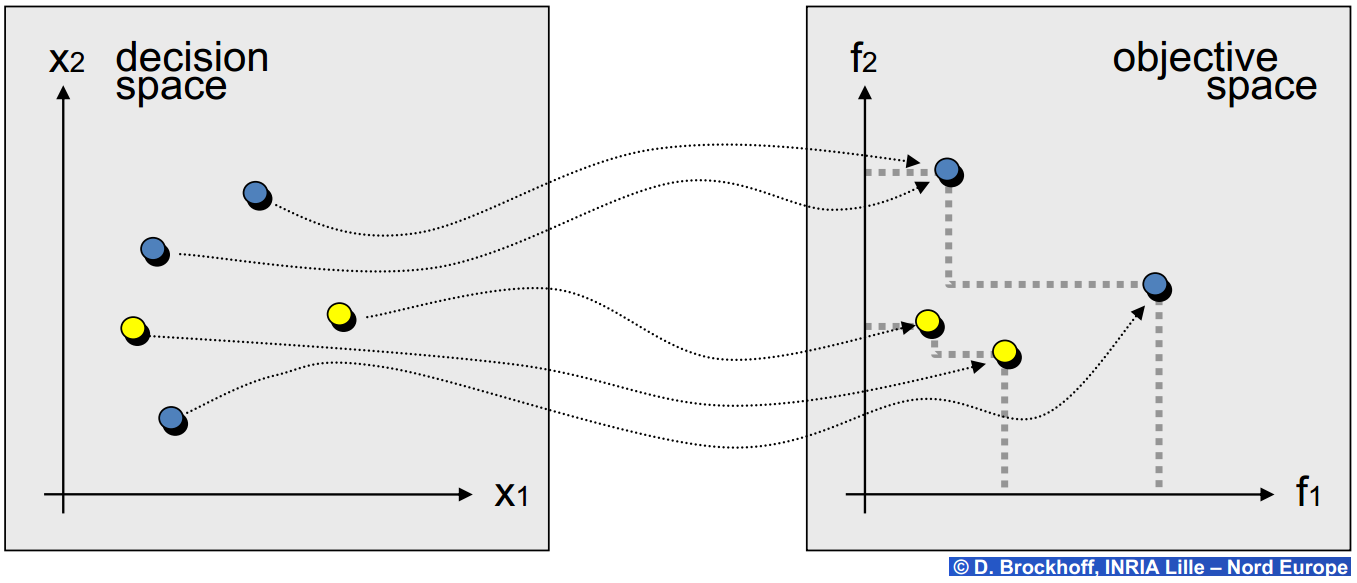
\includegraphics[scale=0.235]{img/moopDec.png}
	\caption{Decision and objective spaces in a MOOP with two variables ($x_1$ and $x_2$) and two objectives ($f_1$ and $f_2$). In the objective space, yellow dots are non-optimal objective vectors, while blue dots form a non-dominated set.}
	\label{fig:moop}
	\end{center}
\end{figure}

There are many different algorithms in the litrature which are proposed to tackle multi-objective optimization problems~\cite{Deb2001}. Weighted-sum approach is one of the traditional methods in which the objectives are weighted according to user preference. The sum of the weighted objectives builds one objective function which is to be optimized. The solution to this single-objective problem is one certain solution, ideally on a Pareto-front. By varying the weights, it is possible to converge to different optimal solutions. Such linear scalarization approaches fail to find optimal solutions for problems with non-convex-shape Pareto-fronts~\cite{Deb2001}.


A popular choice for multi-objective optimization problems are evolutionary multi-objective optimization (EMO) algorithms~\cite{Coello1999, Zhou2011}. 
The goal of EMO algorithms is to find a set of optimal solutions with a good convergence to the Pareto-front as well as a good spread and diversity along the Pareto-front.
One of the most well-known algorithms in the literature is the Non-dominated Sorting Evolutionary Algorithm II (NSGA-{II})~\cite{Deb2002}, pseudocode of which is shown in Algorithm~\ref{alg:nsga2}. As in any evolutionary algorithm, NSGA-{II} evolves a set of $N$ individuals in a population denoted as $Pop$ with the difference that they are ranked according to dominance criterion and a crowding distance measure which is used to maintain a good diversity of solutions.  

\begin{algorithm}[!t]
\begin{algorithmic}[1]
%\Function{NSGA-{II}}{}
\State \textbf{Input:} MOP, N
\State \textbf{Output:} Non-dominated Set $F_0$
	\State $t = 0$
	\State $Pop(t) = NewRandomPopulation$	
	\State $Q(t) = breed (Pop(t))$ \% Generate offspring
	\While{Termination criterion not met}
		\State $U(t) = Pop(t) \cup Q(t)$
		\State $F = \Call{fastNonDominatedSort}{U(t)}$
	    \State $Pop(t+1) = \emptyset$, $i = 0$		
		\While{$|Pop(t+1)|+ |F_i| \leq N$}
			\State $\Call{crowdingDistanceAssignment}{F_i}$	
			\State $Pop(t+1) = Pop(t+1) \cup F_i$
			\State $i = i+1$
		\EndWhile
		\State $\Call{sort}{Pop(t+1)}$
		\State $Pop(t+1) = Pop(t+1) \cup F_i[1:(N-|Pop(t+1)|)]$
		\State $Q(t+1) = breed(Pop(t+1))$	
		\State $t = t+1$
	\EndWhile
	\Return $F_0$
%\EndFunction
\end{algorithmic}
\caption{NSGA-{II} Algorithm \cite{Deb2002}}
\label{alg:nsga2}
\end{algorithm}

The three main pillars of the NSGA-2 algorithm are:
\begin{itemize}
\item Fast non-dominated sorting: The function $F = \Call{fastNonDominatedSort}{U(t)}$ performs a non-dominated sorting and ranks the individuals stored in a set $U$ into several non-dominated fronts denoted as $F_i$, where the solutions in $F_0$ are the non-dominated solutions in the entire set. $F_i$ is the set of non-dominated solutions in $R \setminus (F_0 \cup \cdots \cup F_{i-1})$. 
\item Crowding distance: The function $\Call{crowdingDistanceAssignment}{F_i}$ assigns to each one of the individuals in $F_i$ a crowding distance value, which is the distance between the individual and its neighbours. The individuals with the smallest crowding distances are selected with a lower probability than the ones with the larger values.  
\item Elitism: The solutions in the first front $F_0$ always survive to the next population. 
\end{itemize}


%%%%%%%%%%%%%
% DO WE NEED THIS AT ALL??? 
%A more recent approach called Multi-Objective Evolutionary Algorithm based on Decomposition (MOEA/D)~\cite{Zhang2007} is a combination of traditional linear scalirization approach and EMO. This approach is decomposes the MOP into several single-objective optimization sub-problems and an evolutionary algorithm optimizes them all simultaneously. Information is shared between neighbouring sub-problems in order to guide evolution. 
%The authors show that MOEA/D performs similarly than, and sometimes even outperforms, NSGA-II in the scenarios tested.
%%%%%%%%%%%%%
For more details about EMO approaches, please refer to \cite{Deb2001}.

\subsection{Multi-objective Reinforcement Learning (MORL)}

Reinforcement Learning (RL) algorithms have also been used with MOPs. RL~\cite{Sutton1998} is a broad field in Machine Learning that studies real-time planning and control situations where an agent has to find the actions (or sequences of actions) that should be used in order to maximize the reward from the environment. 

The dynamics of an RL problem are usually captured by a Markov Decision Process (MDP) which is a tuple $(S, A, T, R)$, where $S$ is the set of possible states in the problem (or game), and $s_0$ is the initial state. $A$ is the set of available actions the agent can make at any given time, and the transition model $T(s_i, a_i, s_{i+1})$ determines the probability of reaching the state $s_{i+1}$ when action $a_i$ is applied in state $s_i$. The reward function $R(s_i)$ provides a single value (\textit{reward}) that the agent must optimize, representing the desirability of the state $s_i$ reached. Finally, a policy $\pi(s_i) = a_i$ determines which actions $a_i$ must be chosen from each state $s_i \in S$\footnote{This is a deterministic policy and only valid during acting, not learning}. One of the most important challenges in RL, as shown in Section~\ref{sec:mcts}, is the trade-off between exploration and exploitation while trying to act. While learning, a policy must choose between selecting the actions that provided good rewards in the past and exploring new parts of the search space by selecting new actions. 

Multi-objective Reinforcement Learning (MORL)~\cite{Vamplew2010} changes this definition by using a vector $R = {r_1, \dots, r_m}$ as rewards of the problem (instead of a scalar). Thus, MORL problems differ from RL in having more than one objective (here $m$) that must be maximized. If the objectives are independent or non-conflicting, scalarization approaches such as weighted sum approach, could be suitable to tackle the problem. Essentially, this would mean using a conventional RL algorithm on a single objective where the global reward is obtained from a weighted-sum of the multiple rewards. However, this is not always the case, as usually the objectives are conflicting and the policy $\pi$ must balance among them.

Vamplew et al.~\cite{Vamplew2010} propose a \textit{single-policy} algorithm which uses a preference order in the objectives (either given by the user or by the nature of the problem). 
An example of this type of algorithm can be found at~\cite{Gabor1998}, where the authors introduce an order of preference in the objectives and constrain the value of the desired rewards. Scalarization approaches would also fit in this category, as shown in the work performed by S. Natarajan et al.~\cite{Natarajan2005}.

The second type of algorithms, \textit{multiple-policy}, aims to approximate the optimal Pareto-front of the problem. This is the aim of the algorithm proposed in this paper. An example of this type of algorithm is the one given by L. Barrett~\cite{Barrett2008}, who proposes the Convex Hull Iteration Algorithm. This algorithm provides the optimal policy for any linear preference function, by learning all policies that define the convex hull of the Pareto-front.



\subsection{Metrics}
The quality of an obtained non-dominated set can be measured using different diversity or/and convergence metrics~\cite{Deb2001}. The Hypervolume Indicator (HV) is a popular metric for measuring both the diversity and convergence of non-dominated solutions~\cite{Zitzler-Smetric}. This approach can be additionally used to compare different non-dominated sets. 
Given a Pareto front $P$, $HV(P)$ is defined as the volume of the objective space dominated by $P$. More formally, $HV(P) = \mu (x \in \mathbb{R}^{d} : \exists r \in P \hspace{0.25cm} s.t \hspace{0.25cm} r \preceq x)$, where $\mu$ is the de Lebesgue measure on $\mathbb{R}^{d}$. If the objectives are to be maximized, the higher the $HV(P)$, the better the front calculated. Figure~\ref{fig:hv} shows an example of $HV(P)$ where the objective dimension space is $m=2$.

%%%%%%%%%%%%%%%%%%%%%%%%%%
% I DON'T GET HOW DO WE DO THIS:  $HV(P) = \mu (x \in \mathbb{R}^{d} : \exists r \in P \hspace{0.25cm} s.t \hspace{0.25cm} r \preceq x)$ ????????????????
%%%%%%%%%%%%%%%%%%%%%%%%%%


\begin{figure}[!t]
\begin{center}
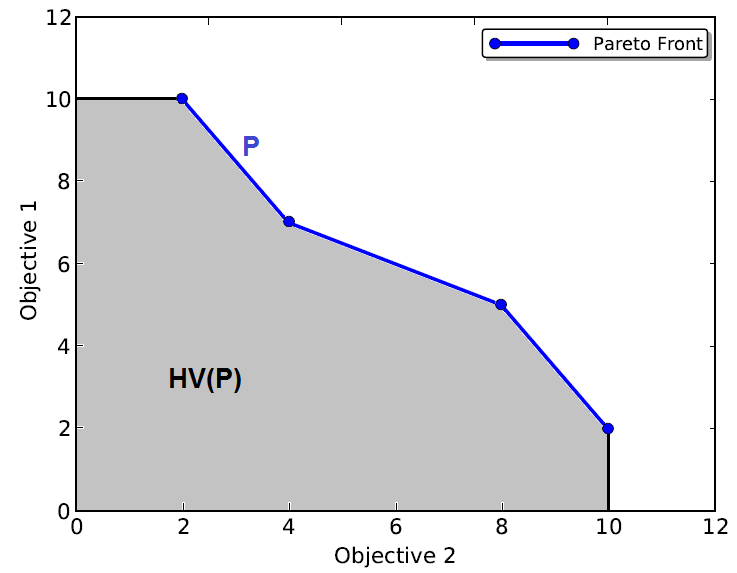
\includegraphics[width=0.75\columnwidth]{img/hv}
\end{center}
\caption{$HV(P)$ of a given Pareto-front $P$}
\label{fig:hv}
\end{figure}



\section{Multi-Objective Monte Carlo Tree Search} \label{sec:momcts}

Adapting MCTS into Multi-Objective Monte Carlo Tree Search (MO-MCTS) requires the obvious modification of dealing with multiple rewards instead of just one. As these are collected at the end of a Monte Carlo simulation, the reward value $r$ now becomes a vector $R = {r_0, r_1, \dots, r_m}$, where $m$ is the number of objectives to optimize. Derived from this change, the average value $Q(s,a)$ becomes a vector that stores the average reward of each objective. Note that the other statistics ($N(s,a)$ and $N(s)$) do not need to change, as these are just node and action counters. The important question to answer next is how to adapt the vector $Q(s,a)$ to use it in the UCB1 formula (Equation~\ref{eq:ucb1}). 

An initial attempt at Multi-Objective MCTS was addressed by W. Wang and Michele Sebag~\cite{Weijia2012, Weijia2013}. In their work, the authors employ a mechanism, based on the HV calculation, to replace the UCB1 equation. The algorithm keeps a Pareto archive (P) with the best solutions found in end game states. Every node in the tree defines $\overline{r}_{sa}$ as a vector of UCB1 values, in which each $\overline{r}_{sa, i}$ is the result of calculating UCB1 for each particular objective $i$.

The next step is to define the value for each state and action pair, $V(s,a)$, as in Equation~\ref{eq:wang}. $\overline{r}^p_{sa}$ is the projection of $\overline{r}_{sa}$ into the piecewise linear surface defined by the Pareto archive $P$ (see Figure~\ref{fig:wangHV}). Then, $HV(P \cup \overline{r}_{sa})$ is declared as the HV of $P$ plus the point $\overline{r}_{sa}$. If $\overline{r}_{sa}$ is dominated by P, the distance between $\overline{r}_{sa}$ and $\overline{r}^p_{sa}$ is subtracted from the HV calculation. The tree policy selects actions based on a maximization of the value of $V(s,a)$.

\begin{equation} \label{eq:wang}
	V(s,a) = \left\{
\begin{array}{l l}      
    HV(P \cup \overline{r}_{sa}) - dist(\overline{r}^p_{sa}, \overline{r}_{sa} )\hspace{0.5cm} Otherwise \\
    HV(P \cup \overline{r}_{sa}) \hspace{0.5cm} if \hspace{0.25cm} \overline{r}_{sa} \preceq P\\
\end{array}\right.
\end{equation}


\begin{figure}[!t]
\begin{center}
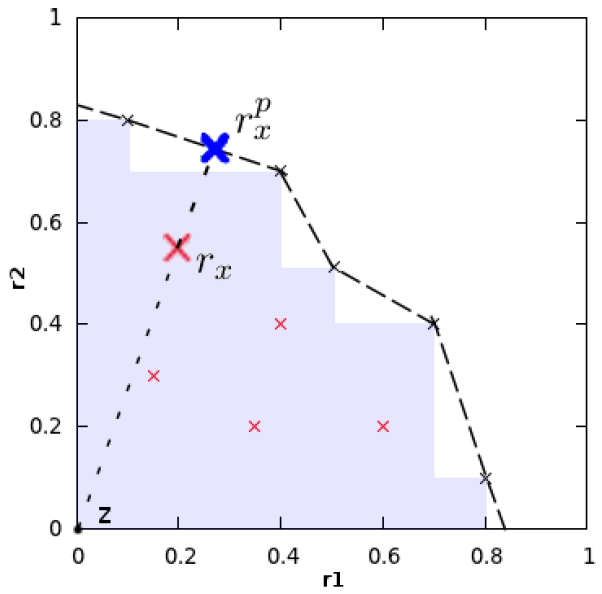
\includegraphics[width=0.65\columnwidth]{img/wangHV}
\end{center}
\caption{$r^p_x$ is the projection of the $r_x$ value on the piecewise linear surface (discontinuous line). The shadowed surface represents $HV(P)$. From~\cite{Weijia2012}.}
\label{fig:wangHV}
\end{figure}
 
The proposed algorithm was employed successfully in two domains: the DST and the Grid Scheduling problem, matching state-of-the-art results in both cases, at the expense of a high computational cost.

As mentioned before, the objective of this paper is to propose an MO-MCTS algorithm that is suitable for real-time domains. Although the work discussed here is influenced by Wang's approach, some modifications need to be done in order to overcome the high computational cost involved in their approach.

In the algorithm proposed in this paper, the reward vector $\overline{r}$ that was obtained at the end of a Monte Carlo simulation is back-propagated through the nodes visited in the last iteration until the root is reached. In the vanilla algorithm, each node would use this vector $\overline{r}$ to update its own accumulated reward vector $\overline{R}$. In the algorithm proposed here, each node in the MO-MCTS algorithm also keeps a local Pareto front ($P$), updated at each iteration with the reward vector $\overline{r}$ obtained at the end of the simulation. Algorithm~\ref{alg:updPareto} describes how the node statistics are updated in MO-MCTS.

\begin{algorithm}[!t]
\begin{algorithmic}[1]
\Function{Update}{$node, \overline{r}, dominated=false$}

	\State $node.Visits = node.Visits + 1$
	\State $node.\overline{R} = node.\overline{R} + \overline{r}$
	\If{$!dominated$} 
		\If{$node.P \preceq \overline{r}$}	
			\State $dominated = true$
		\Else
			\State $node.P = node.P \cup \overline{r}$
		\EndIf
	\EndIf

	\State $\Call{Update}{node.parent,\overline{r},dominated}$
	
\EndFunction
\end{algorithmic}
\caption{Pareto MO-MCTS node update.}
\label{alg:updPareto}
\end{algorithm}

Here, if $\overline{r}$ is not dominated by the local Pareto front, it is added to the front and $\overline{r}$ is propagated to its parent. In case $\overline{r}$ is dominated by the node's Pareto front, the local Pareto front does not change and there is no need to keep this propagation up the tree. Three observations can be made about the mechanism described here:

\begin{itemize}
\item Each node in the tree has an estimate of the quality of the solutions reachable from there, both as an average (as in the baseline MCTS) and as the best case scenario (by keeping the non-dominated front $P$).
\item By construction, if a reward $\overline{r}$ is dominated by the local front of a node, it is a given that it will be dominated by the nodes above in the tree, so there is no need to update the fronts of the upper nodes, producing little impact on the computational cost of the algorithm.
\item It is easy to infer, from the last point, that the Pareto front of a node cannot be worse than the front of its children (in other words, the front of a child will never dominate that of its parent). Therefore, the root of the tree contains the best non-dominated front ever found during the search.
\end{itemize}

This last detail is important for two main reasons. First of all, the algorithm allows the root to store information as to which action to take in order to converge to any specific solution in the front discovered. This information can be used, when all iterations have been performed, to select the move to perform next. If weights for the different objectives are provided, these weights can be used to select the desired solution in the Pareto front of the root node, and hence select the action that leads to that point. Secondly, the root's Pareto front can be used to measure the global quality of the search using the hypervolume calculation.

Finally, the information stored at each node regarding the local Pareto front can be used to substitute $Q(s,a)$ in the UCB1 equation. The quality of a given pair $(s,a)$ can be obtained by measuring the HV of the Pareto front stored in the node reached from state $s$ after applying action $a$. This can be defined as  $Q(s,a) = HV(P)/N(s)$, and the Upper Confidence Bound equation, referred to here as $MO-UCB$, is described as in Equation~\ref{eq:moucb}). 

\begin{equation}	\label{eq:moucb}
a^* = \argmax_{a \in A(s)} \left\{HV(P)/N(s) + C \sqrt{\frac{ \ln N(s) }{ N(s,a) }}\right\}
\end{equation}

This algorithm, similar to NSGA-II due to their multi-objective nature, provides a non-dominated front as a solution. However, in planning and control scenarios like the games analyzed in this research, an action must be provided to perform a move in the next step. The question that arises is how to choose the move to make based on the information available.

As shown before, it is straightforward to discover which actions lead to what points in the front given as a solution: first gene in the best NSGA-II individual, a root's child in MO-MCTS. Hence, by identifying the point in the Pareto front that the algorithm should converge to, 
it is possible to execute the action that leads to that point.

In order to select a point in the Pareto front, a weight vector $W$ can be defined, with a dimension $m$ equal to the number of objectives ($W = (w_1, w_2, \dots, w_m); \sum_{i}^{m} w_i = 1$). Two different mechanisms are proposed, for reasons that will be explained in the experiments section (\ref{sec:exp}):

\begin{itemize}
\item Weighted Sum: the action chosen is the one that maximizes the weighted sum of the reward vector multiplied by $W$, for each point in the front.
\item Euclidean distance: the euclidean distance from each point in the Pareto front (normalized in $[0,1]$) to the vector $W$ is calculated. The action to choose would be the one that leads to the point in the Pareto front with the shortest distance to $W$. 
\end{itemize}

Note that, in the vanilla MCTS, there is no Pareto front obtained as a solution. Typically, in this case, rewards are calculated as a weighted sum of the objectives and a weight vector $W$, and then the action is chosen following any of the mechanisms usually employed in the literature: the action taken more often from the root; the one that leads to the best reward found; the move with the highest expected reward; or the action that maximizes Equation~\ref{eq:ucb1} in the root.

\section{Benchmarks} \label{sec:bench}

Two different games are used in this research to analyze the performance of the algorithm proposed.

\subsection{Deep Sea Treasure} \label{ssec:dst}

The Deep Sea Treasure (DST) is a popular multi-objective problem introduced by Vamplew et al.~\cite{Vamplew2010}. In this single-player puzzle, the agent controls a submarine with the objective of finding a treasure located at the bottom of the sea. The world is divided into a grid of $10$ rows and $11$ columns, and the vessel starts at the top left board position. There are three types of cells: empty cells (or water), that the submarine can traverse; ground cells that, as the edges of the grid, cannot be traversed; and treasure cells, that provide different rewards and finish the game. Figure~\ref{fig:dstBase} shows the DST environment.

\begin{figure}[!t]
\begin{center}
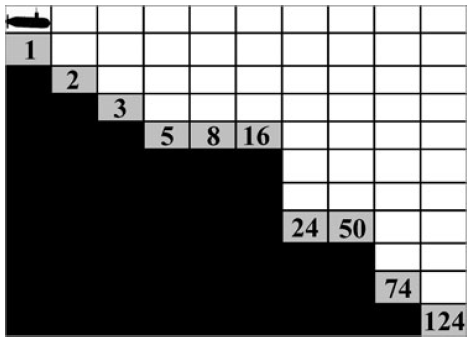
\includegraphics[width=0.75\columnwidth]{img/dst}
\end{center}
\caption{Environment of the Deep Sea Treasure (from~\cite{Vamplew2010}): grey squares represent the treasure (with their different values) available in the map. The black cells are the sea floor and the white ones are the positions that the vessel can occupy freely. The game ends when the submarine picks one of the treasures.}
\label{fig:dstBase}
\end{figure}


The ship can perform four different moves: \textit{up}, \textit{down}, \textit{right}  and \textit{left}. If the action applied takes the ship off the grid or into the sea floor, the vessel's position does not change.  There are two objectives in this game: the number of moves performed by the ship, that must be minimized, and the value of the treasure found, that should be maximized. As can be seen in Figure~\ref{fig:dstBase}, the most valuable treasures are at a greater distance from the initial position, so the objectives are in conflict.

Additionally, the agent can only make up to $100$ plies or moves. This allows the problem to be defined as the maximization of two rewards: $(\rho_p,\rho_v) = (100 - plies, treasureValue)$. Should the ship perform all moves without reaching a treasure, the result would be ($0$,$0$). At each step, the score of a location with no treasure is ($-1$, $0$).

The optimal Pareto front of the DST is shown in Figure~\ref{fig:optDst}. There are $10$ non-dominated solutions in this front, one per each treasure in the board. The front is globally concave, with local concavities at the second $(83,74)$, fourth $(87,24)$ and sixth $(92,8)$ points from the left. The HV value of the optimal front is $10455$.

\begin{figure}[!t]
\begin{center}
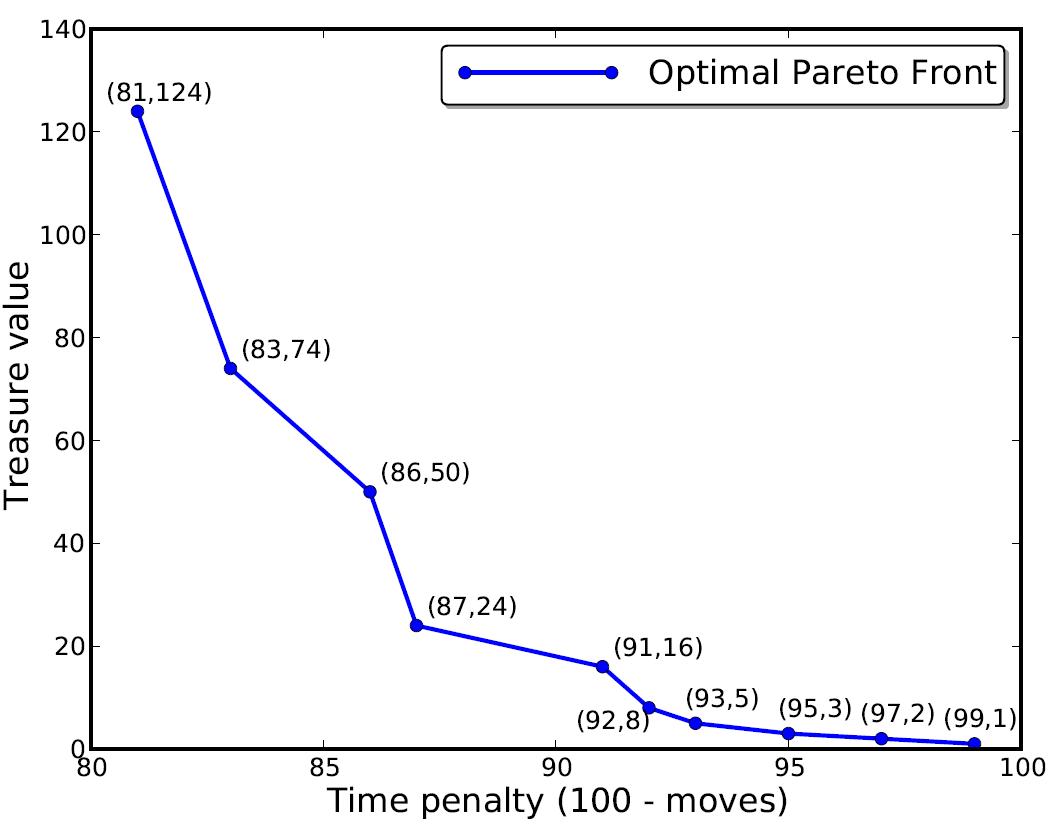
\includegraphics[width=1.0\columnwidth]{img/optDST.png}
\end{center}
\caption{Optimal Pareto Front of the Deep Sea Treasure, with both objectives to be maximized.}
\label{fig:optDst}
\end{figure}

Section~\ref{sec:moo} introduced the problems of linear scalarization approaches when facing non-convex optimal Pareto fronts. The concave shape of the DST's optimal front means that those approximations converge to the non dominated solutions located at the edges of the Pareto front: $(81,124)$ and $(99,1)$. Note that this happens independently from the weights chosen for the linear approximation: some solutions of the front just can't be reached with these approaches. Thus, successful approaches should be able to find all elements of the optimal Pareto front and converge to any of the non dominated solutions.

\subsubsection{Transposition Tables in DST} \label{ssec:transTables}

The DST is a problem specially suited for the use of Transposition Tables (TT)~\cite{Childs2008} within MCTS. TT is a technique used to optimize three search based algorithms when two or more states can be found at different locations in the tree. It consists of sharing information between these equivalent states in a centralized manner, in order to avoid managing these positions as completely different states. Figure~\ref{fig:dstTable} shows an example of this situation in the DST.

\begin{figure}[!t]
\begin{center}
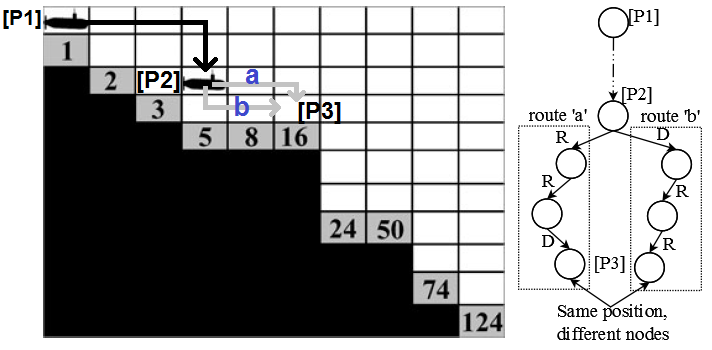
\includegraphics[width=0.9\columnwidth]{img/dstTransTables}
\end{center}
\caption{Example of two different sequences of actions (R: Right, D: Down) that lie in the same position in the map, but at a different node in the tree.}
\label{fig:dstTable}
\end{figure}

In this example, the submarine starts in the initial position ($P1$, root of the tree) and makes a sequence of moves that places it in $P2$. From this location, two optimal trajectories to move to $P3$ would be route \textit{a} and \textit{b}. In a tree that does not use TT, there would be two different nodes to represent $P3$, although the location and number of moves performed up to this point are the same (thus, the states are equivalent). It is worthwhile highlighting that the coordinates of the vessel are not enough to identify two equivalent states, the number of moves is also needed: imagine a third route from $P2$ to $P3$ with the moves: \textit{Up}, \textit{Right}, \textit{Right}, \textit{Down}, \textit{Down}. As the submarine performs $5$ moves, the states are not the same, and the node where the ship is in $P3$ now would be two levels deeper in the tree.

TT tables are implemented in the MCTS algorithms tested in this benchmark by using hash tables that store a \textit{representative} node for each pair $(position, moves)$ found.  The key of the hash map needs then to be obtained from three values: position coordinates $x$ and $y$ of the ship in the board, and number of moves, indicated by the depth of the node in the tree. Hence, transpositions can only happen at the same depth within the tree, a feature that has been successfully tried before in the literature~\cite{Kozelek2009}.

\subsubsection{Heuristics for DST} \label{sssec:heurDST}

As DST has two different objectives, number of moves and value of the treasure, the quality of a state can be assessed by two rewards, $\rho_p$ and $\rho_v$, for each objective respectively. $\rho_p$ is adjusted to be maximized using the maximum number of moves in the game, while $\rho_v$ is just the value in the cell with the treasure. Equation~\ref{eq:dst} summarizes these rewards:

\begin{equation}	\label{eq:dst}
\begin{split}
\rho_p = 100 - moves \\
\rho_v = treasureValue
\end{split}
\end{equation}


\subsection{Multi-Objective PTSP} \label{ssec:moptsp}

The Multi-Objective Physical Travelling Salesman Problem (MO-PTSP) is a game that was employed in a competition held at the IEEE Conference on Computational Intelligence in Games (CIG) in 2013. This was a modification of the Physical Travelling Salesman Problem (PTSP), previously introduced by Perez et al.~\cite{PerezCEC2012}. The MO-PTSP is a real-time game where the agent navigates a ship and must visit $10$ waypoints scattered around the maze. All waypoints must be visited to consider a game as complete, and a game-tick counter is reset every time a waypoint is collected, finishing the game prematurely (and unsuccessfully) if $800$ game steps are reached before visiting another waypoint.

This needs to be done while optimizing three different objectives:  1) \textbf{Time}: the player must collect all waypoints scattered around the maze in as few time steps as possible; 2) \textbf{Fuel}: the fuel consumption by the end of the game must be minimized; and 3) \textbf{Damage}: the ship should end the game with as little damage as possible.

In the game, the agent must provide an action every $40$ milliseconds. The available actions are combinations of two different inputs: \textit{throttle} (that could be \textit{on} or \textit{off}) and \textit{steering} (that could be \textit{straight}, \textit{left} or \textit{right}). This allows for $6$ different actions that modify the ship's position, velocity and orientation. These vectors are kept from one step to the next, keeping the inertia of the ship, and making the navigation task not trivial. 

The ship starts with $5000$ units of fuel, and one unit is spent every time an action supplied has the throttle input \textit{on}. There are, however, two ways of collecting fuel: each waypoint visited grants the ship $50$ more units of fuel; and there are also fuel canisters scattered around the maze that provide $250$ more units.

Regarding the third objective, the ship can suffer damage in two different ways: by colliding with obstacles and driving through lava. In the former case, the ship can collide with normal obstacles (that subtract $10$ units of damage) and specially damaging obstacles ($30$ units). In the latter, lava lakes are abundant in MO-PTSP levels and, in contrast with normal surfaces, they deal one unit of damage for each time step the ship spends over this type of surface. All these subtractions are deducted from an initial counter of $5000$ points of damage.

Figure~\ref{fig:sampleMap} shows an example of an MO-PTSP map, as drawn by the framework. Waypoints not yet visited are painted as blue circles, while those already collected are depicted as empty circles. The green ellipses represent fuel canisters, normal surfaces are drawn in brown and lava lakes are printed as red-dotted yellow surfaces. Normal obstacles are black and damaging obstacles are drawn in red. Blue obstacles are elastic walls that produce no damage to the ship. The vessel is drawn as a blue polygon and its trajectory is traced with a black line.

\begin{figure} [!t]
	\begin{center}
	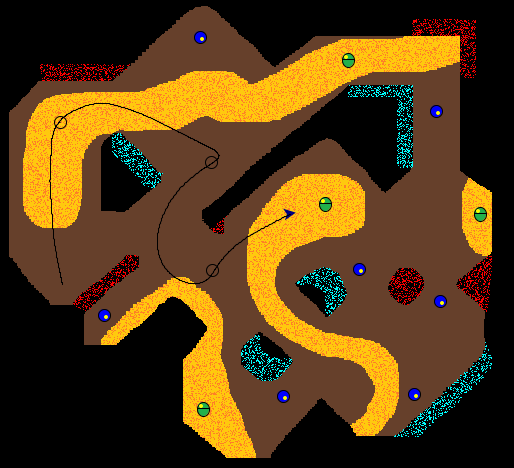
\includegraphics[width=0.8\columnwidth]{img/moptspmap}
	\caption{Sample MO-PTSP map.}
	\label{fig:sampleMap}
	\end{center}
\end{figure}

\subsubsection{Macro-actions for MO-PTSP} \label{sssec:macro}

All algorithms tested in the MO-PTSP in this research employ macro-actions, a concept that can be used for coarsening the action space by applying the action chosen by the control algorithm in several consecutive cycles, instead of just in the next one. 

Previous research in PTSP~\cite{Perez2013, Perez2012} suggests that using macro-actions for real-time navigation domains increases the performance of the algorithms, and it has been used in the previous PTSP competitions by the winner and other entries.

A macro-action of length $L$ is defined as a repetition of a given action during $L$ consecutive time steps. The main advantage of macro-actions is that the control algorithms can see further in the future, and then reduce the implication of open-endedness in real-time games (see Section~\ref{sec:mcts}). As this reduces the search space significantly, a better algorithm performance is allowed. A consequence of using macro-actions is also that the algorithm can employ $L$ consecutive steps to plan the next move (the next macro-action) to make. Therefore, instead of spending $40$ milliseconds, as in MO-PTSP, to define the next action, the algorithm can employ $40 \times L$ milliseconds for this task, and hence perform a more extensive search. 

In MO-PTSP, the macro-action size is $L = 15$, a value that has shown its proficiency before in PTSP. For more information about macro-actions and their application to real-time navigation problems such as the PTSP, the reader is referred to~\cite{Perez2013}.

\subsubsection{Heuristics for MO-PTSP} \label{sssec:heurMOPTSP}

In order to evaluate a game state in MO-PTSP, three different measures or rewards are taken, $\rho_t, \rho_f, \rho_d$, one for each one of the objectives: time, fuel and damage, respectively. All these rewards are defined so they have to be maximized. The first reward uses a measure of distance for the time objective, as indicated in Equation~\ref{eq:dist}: 

\begin{equation}	\label{eq:dist}
\rho_t = 1 - d_t/d_M
\end{equation}

The MO-PTSP framework includes a path-finding library that allows controllers to query the shortest distance of a route of waypoints. $d_t$ indicates the distance from the current position until the last waypoint, following the desired route, and $d_M$ is the distance of the whole route from the starting position. Minimizing the distance to the last waypoint will lead to the end of the game.

Equation~\ref{eq:fuel} shows how the value of the fuel objective, $\rho_f$, is obtained:

%f_p = fuelPoints
%f_c = fuelConsumed
%f_0 = initialFuel

\begin{equation}	\label{eq:fuel}
\rho_f = (1 - (\lambda_t/\lambda_0)) \times \alpha + \rho_t \times (1 - \alpha)
\end{equation}

$\lambda_t$ is the fuel consumed so far, and $\lambda_0$ is the initial fuel at the start of the game. $\alpha$ is a value that balances between the fuel component and the time objective from Equation~\ref{eq:dist}. Note that, as waypoints need to keep being visited, it is necessary to include a distance measure for this reward. Otherwise, an approach that prioritizes this objective would not minimize distance to waypoints at all (the ship could just stand still: no fuel consumed is optimal), and therefore could not complete the game. The value of $\alpha$ has been determined empirically, in order to provide a good balance between these two components, and it is set to $0.66$.

Finally, Equation~\ref{eq:dam} gives the method to calculate the damage objective, $\rho_d$:

%d_p = damagePoints
%d_s = damageSuffered
%d_m = maximumDamage
%s = shipSpeed

\begin{equation}	\label{eq:dam}
\rho_d = 
\begin{cases}
	(1 - (g_t/g_M)) \times \beta_{1} + \rho_t \times (1 - \beta_{1}), & sp > \gamma\\
	(1 - (g_t/g_M)) \times \beta_{2} + \rho_t \times (1 - \beta_{2}), & sp \leq \gamma
\end{cases}
\end{equation}

$g_t$ is the damage suffered so far in the game, and $g_M$ is the maximum damage the ship can take. In this case, three different variables are used to regulate the behaviour of this objective: $\gamma$, $\beta_{1}$ and $\beta_{2}$. Both $\beta_{1}$ and $\beta_{2}$ have the same role as $\alpha$ in Equation~\ref{eq:fuel}: they balance between the time objective and the damage measure. The difference is that $\beta_{1}$ is used in high speeds, while $\beta_{2}$ is employed with low velocities. This is distinguished by the parameter $\gamma$, that can be seen as a threshold value for the ship's speed ($sp$). This differentiation is made in order to avoid low speeds in lava lakes, as this increase the damage suffered significantly. The values for these variables have also been determined empirically, and they are set to $\gamma = 0.8$, $\beta_{1} = 0.75$ and $\beta_{2} = 0.25$.

It is important to highlight again that these three rewards, $\rho_t$, $\rho_f$ and $\rho_d$, are the same for the three algorithms tested in the experiments. 

\section{Experimentation} \label{sec:exp}

The experiments performed in this research compare three different algorithms in the two benchmarks presented in Section~\ref{sec:bench}: a single objective MCTS (referred to here simply as \textit{MCTS}), the Multi-Objective MCTS (\textit{MO-MCTS}) and a rolling horizon version of the NSGA-II algorithm described in Section~\ref{sec:moo} (\textit{NSGA-II}). This NSGA-II version evolves a population where the individuals are sequences of actions (macro-actions in the MO-PTSP case), obtaining the fitness from the state of the game after applying the sequence. The populations sizes, determined empirically, were set to $20$ and $50$ individuals for DST and MO-PTSP respectively. The value of $C$ in Equation~\ref{eq:ucb1} and~\ref{eq:moucb} is set to $\sqrt{2}$.

All algorithms have a limited number of evaluations before providing an action to perform. In order for these games to be real-time, the time budget allowed is close to $40$ milliseconds. With the objective of avoiding congestion peaks at the machine where the experiments are run, the average number of evaluations possible in $40$ ms is calculated and employed in the tests. This leads to $4500$ evaluations in the DST, and $500$ evaluations for MO-PTSP, using the same server where the PTSP and MO-PTSP competitions were run\footnote{Intel Core i5, 230GHz, 4GB of RAM.}.


\subsection{Results in DST} \label{ssec:resDST}

As the optimal Pareto front of the DST is known, a measure of performance can be obtained by observing the percentage of times these solutions are found by the players. As the solution that the algorithms converge to depends on the weights vector employed during the search (see end of Section~\ref{sec:momcts}), the approach taken here is to provide different weight vectors $W$ and analyze them separately.  

The weight vector for DST has two dimensions. This vector is here referred to as $W = (w_p, w_v)$, where $w_p$ weights moves; and $w_v$ weights the treasure value ($w_v = 1 - w_p$). $w_p$ takes values between $0$ and $1$, with a precision of $0.01$, and $100$ experiments have been run for each pair $(w_p, w_v)$. Hence, the game has been played a total of $10000$ times, for each algorithm.


\begin{figure*}[!t]
	\centering
	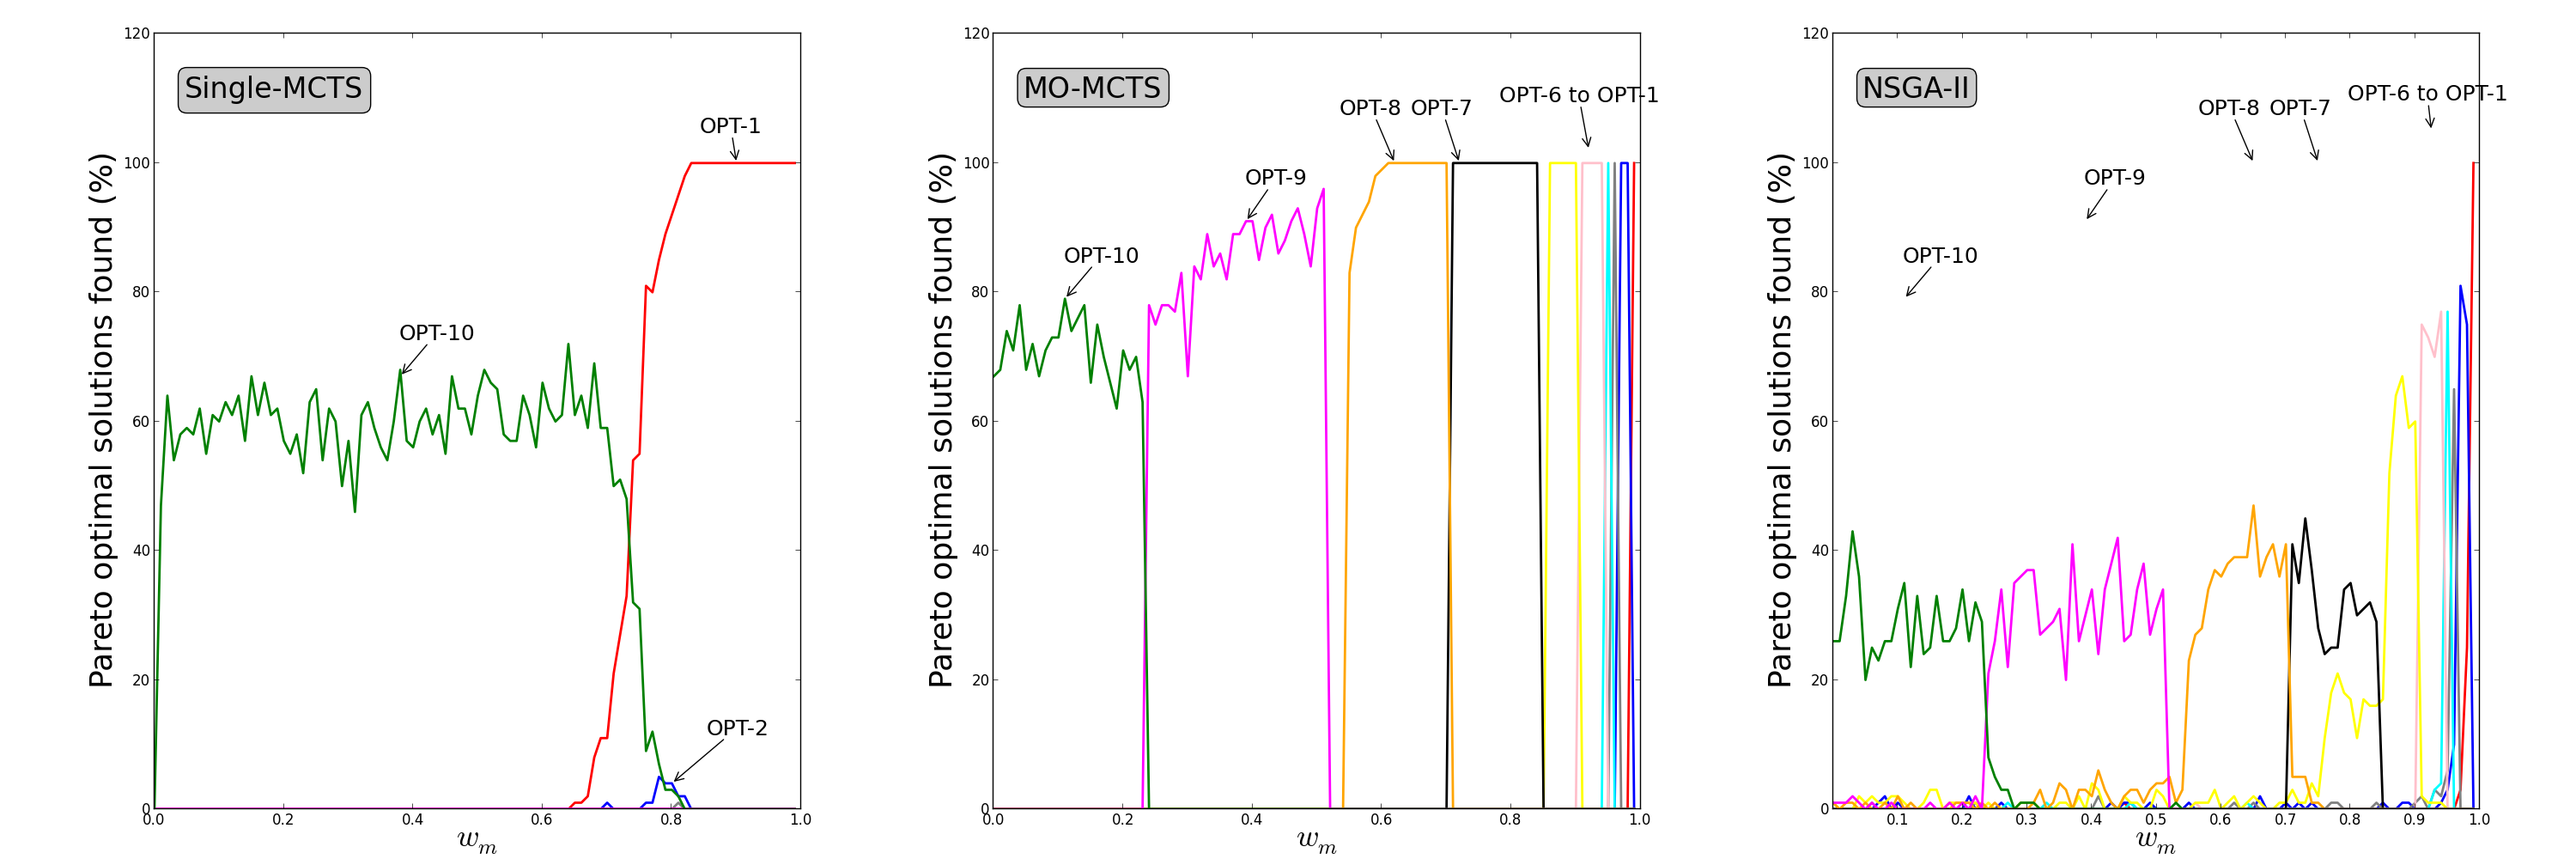
\includegraphics[width=2.1\columnwidth]{img/dstAll}
	\caption{Results in DST: percentages of each optima found during $100$ games played with different weight vectors. Scalarization approaches converge to the edges of the optimal front, whereas Pareto approaches are able to find all optimal solutions. The proposed algorithm, MO-MCTS, finds these solutions significantly more often than NSGA-II.}
	\label{fig:extCase}
\end{figure*}

Figure~\ref{fig:extCase} shows the results obtained after these experiments were performed. The first point to note is that MCTS only converges (mostly) to the two optimal points located at the edges of the optimal Pareto front (\textit{OPT-1} and \textit{OPT-10}, see also Figure~\ref{fig:optDst}). This is an expected result, as K. Deb. suggested in~\cite{Deb2001} and was also discussed before in Section~\ref{sec:moo}: linear scalarization approaches only converge to the edges of the optimal Pareto front if its shape is non-convex.

The results show clearly how approximating the optimal Pareto front allows for finding all possible solutions. Both NSGA-II and MO-MCTS approaches are able to converge to any solution in the front given the appropriate weight vector. It is important to highlight that these two algorithms employed the euclidean distance action selection (see Section~\ref{sec:momcts}). Other experiments, not included in this paper, showed that weighted sum action selection provides similar results to MCTS (that is, convergence to the edges of the front). The crucial distinction to make here is that both algorithms, NSGA-II and MO-MCTS, allow for better action selection mechanisms, that are able to overcome this problem by approximating a global Pareto front.

Finally, in the comparison between NSGA-II and MO-MCTS, the latter algorithm obtains higher percentages for each one of the points in the front. This result suggests that, with a limited number of iterations/evaluations, the proposed algorithm is able to explore the search space more efficiently than a rolling horizon version of a state-of-the-art NSGA-II.


\subsection{Results in MO-PTSP} \label{ssec:resMOPTSP}

The same three algorithms have been tested in the MO-PTSP domain. The experiments are performed in the $10$ maps available within the framework~\footnote{Available at \url{www.ptsp-game.net}}. In this case, the optimal Pareto front is not known in advance, and normally it will differ from one map to another. Hence, the mechanisms to compare the performance of the algorithms tested need to be different than the one used for DST.

The idea is as follows. First of all, $4$ different weight vectors are tested: $W_1 = (0.33,0.33,0.33)$, $W_2 = (0.1,0.3,0.6)$, $W_3 = (0.1,0.6,0.3)$ and $W_4 = (0.6,0.1,0.3)$, where each $w_i$ corresponds to the weight for an objective ($w_t$ for time, $w_f$ for fuel and $w_d$ for damage, in this order). $W_1$ treats all objectives with the same weight, while the other three give more relevance to different objectives. These vectors then provide a wide spectrum for weights in this benchmark. In this case, MO-MCTS uses these weights to select an action based on a weighted sum, which in preliminary experiments has shown better performance than the Euclidean distance mechanism.

The first point to check is if the different weight vectors affect the solutions obtained by MO-MCTS. Table~\ref{tab:weights} shows the results of executing the MO-MCTS controller during $30$ games in each one of the $10$ maps of the MO-PTSP, for every weight vector. It can be seen that the highest weight in $W$ leads, in most of the cases, to the best solution in that objective in the map. 


\begin{table}[!t]
\begin{center}
%\begin{tabular}{|>{\centering\arraybackslash}m{0.65cm}|c|c|c|c|}
\begin{tabular}{|p{0.8cm}|p{2.2cm}|m{1.13cm}|m{1.13cm}|m{1.13cm}|}
\hline
\textbf{Map}  & \textbf{$W:(w_t, w_f, w_d)$} & \textbf{Time} &  \textbf{Fuel} & \textbf{Damage} \\ 
\hline
 \multirow{3}{*}{\textbf{Map 1}} & $(0.33,0.33,0.33)$ & $1654 \pm 7$ & $131 \pm 2$& $846 \pm 13$\\
 & $(0.1,0.3,0.6)$ & $1657 \pm 8$ & $130 \pm 2$ & \bm{$773 \pm 11$}\\
 & $(0.1,0.6,0.3)$ & $1681 \pm 11$ & $131 \pm 2$ & $837 \pm 15$\\
 & $(0.6,0.1,0.3)$ & \bm{$1649 \pm 8$} & $132 \pm 2$ & $833 \pm 13$\\
\hline
 \multirow{3}{*}{\textbf{Map 2}} & $(0.33,0.33,0.33)$ & $1409 \pm 7$ & $235 \pm 4$& $364 \pm 3$\\
 & $(0.1,0.3,0.6)$ & $1402 \pm 6$ & $236 \pm 5$ & \bm{$354 \pm 2$}\\
 & $(0.1,0.6,0.3)$ & $1416 \pm 8$ & \bm{$219 \pm 4$} & $360 \pm 3$\\
 & $(0.6,0.1,0.3)$ & $1396 \pm 8$ & $245 \pm 5$ & $361 \pm 2$\\
\hline
 \multirow{3}{*}{\textbf{Map 3}} & $(0.33,0.33,0.33)$ & $1373 \pm 6$ & $221 \pm 3$& $301 \pm 7$\\
 & $(0.1,0.3,0.6)$ & $1378 \pm 5$ & $211 \pm 3$ & \bm{$268 \pm 5$}\\
 & $(0.1,0.6,0.3)$ & $1385 \pm 6$ & \bm{$203 \pm 4$} & $291 \pm 7$\\
 & $(0.6,0.1,0.3)$ & \bm{$1363 \pm 4$} & $229 \pm 4$ & $285 \pm 7$\\
\hline
 \multirow{3}{*}{\textbf{Map 4}} & $(0.33,0.33,0.33)$ & $1383 \pm 6$ & $291 \pm 5$& $565 \pm 5$\\
 & $(0.1,0.3,0.6)$ & $1385 \pm 7$ & $304 \pm 4$ & \bm{$542 \pm 4$}\\
 & $(0.1,0.6,0.3)$ & $1423 \pm 6$ & \bm{$273 \pm 4$} & $583 \pm 5$\\
 & $(0.6,0.1,0.3)$ & $1388 \pm 6$ & $309 \pm 4$ & $559 \pm 5$\\
\hline
 \multirow{3}{*}{\textbf{Map 5}} & $(0.33,0.33,0.33)$ & $1405 \pm 7$ & $467 \pm 4$& $559 \pm 4$\\
 & $(0.1,0.3,0.6)$ & $1431 \pm 9$ & $447 \pm 4$ & \bm{$541 \pm 4$}\\
 & $(0.1,0.6,0.3)$ & $1467 \pm 9$ & \bm{$411 \pm 5$} & $567 \pm 5$\\
 & $(0.6,0.1,0.3)$ & \bm{$1399 \pm 9$} & $469 \pm 4$ & $547 \pm 3$\\
\hline
 \multirow{3}{*}{\textbf{Map 6}} & $(0.33,0.33,0.33)$ & $1575 \pm 7$ & $549 \pm 5$& $303 \pm 4$\\
 & $(0.1,0.3,0.6)$ & $1626 \pm 9$ & $540 \pm 6$ & \bm{$286 \pm 5$}\\
 & $(0.1,0.6,0.3)$ & $1703 \pm 11$ & \bm{$499 \pm 4$} & $316 \pm 7$\\
 & $(0.6,0.1,0.3)$ & \bm{$1571 \pm 7$} & $559 \pm 5$ & $294 \pm 4$\\
\hline
 \multirow{3}{*}{\textbf{Map 7}} & $(0.33,0.33,0.33)$ & $1434 \pm 5$ & $599 \pm 6$& $284 \pm 6$\\
 & $(0.1,0.3,0.6)$ & $1475 \pm 10$ & $602 \pm 5$ & \bm{$243 \pm 6$}\\
 & $(0.1,0.6,0.3)$ & $1489 \pm 12$ & \bm{$549 \pm 3$} & $264 \pm 6$\\
 & $(0.6,0.1,0.3)$ & \bm{$1407 \pm 8$} & $618 \pm 5$ & $270 \pm 6$\\
\hline
 \multirow{3}{*}{\textbf{Map 8}} & $(0.33,0.33,0.33)$ & $1761 \pm 9$ & $254 \pm 5$& $382 \pm 3$\\
 & $(0.1,0.3,0.6)$ & $1804 \pm 10$ & $269 \pm 4$ & \bm{$357 \pm 4$}\\
 & $(0.1,0.6,0.3)$ & $1826 \pm 10$ & \bm{$230 \pm 3$} & $392 \pm 7$\\
 & $(0.6,0.1,0.3)$ & \bm{$1732 \pm 9$} & $311 \pm 8$ & $379 \pm 6$\\
\hline
 \multirow{3}{*}{\textbf{Map 9}} & $(0.33,0.33,0.33)$ & $2501 \pm 14$ & $926 \pm 6$& $574 \pm 9$\\
 & $(0.1,0.3,0.6)$ & $2503 \pm 10$ & $921 \pm 10$ & \bm{$524 \pm 8$}\\
 & $(0.1,0.6,0.3)$ & $2641 \pm 14$ & \bm{$833 \pm 5$} & $574 \pm 14$\\
 & $(0.6,0.1,0.3)$ & \bm{$2470 \pm 9$} & $956 \pm 5$ & $573 \pm 8$\\
\hline
 \multirow{3}{*}{\textbf{Map 10}} & $(0.33,0.33,0.33)$ & $1430 \pm 8$ & $630 \pm 4$& $205 \pm 2$\\
 & $(0.1,0.3,0.6)$ & $1493 \pm 13$ & $615 \pm 4$ & $209 \pm 2$\\
 & $(0.1,0.6,0.3)$ & $1542 \pm 10$ & \bm{$554 \pm 4$} & $229 \pm 5$\\
 & $(0.6,0.1,0.3)$ & \bm{$1378 \pm 5$} & $663 \pm 6$ & $202 \pm 4$\\
\hline
\end{tabular}
\caption{MO-MCTS results in MO-PTSP with different weight vectors. Significantly better results per map are in bold.}
\label{tab:weights}
\end{center}
\end{table}

Some exceptions can be explained by analysing the map: in map 1, a fuel canister is always collected near the end, restoring the fuel level to its maximum. This leaves too few cycles to make a difference in the controller (note also that this is the map with the smallest fuel consumption). Also, in map 10, there is no difference in the damage objective: but map 10 is a map with no obstacles to damage the ship (thus only lava lakes deal damage). This also results in this map being the one with the lowest overall damage. It can also be seen that, in those maps where time has priority, the results for this objective are not as dominant as the other two. This can be explained by the fact that the time heuristic is actually part of the fuel and damage heuristics (Equation~\ref{eq:dist} in Eqs.~\ref{eq:fuel} and~\ref{eq:dam}).

These results suggest that the weights effectively work on making the algorithm converge to different points in the Pareto front discovered by the algorithm. Now, it is time to compare these results with the other algorithms. In order to do this, the same number of experiments is run for NSGA-II and MCTS in the $10$ maps of the benchmark.

In order to compare the several algorithms, the results are examined in pairs, in terms of dominance. The procedure is as follows: once all games on a single map have been run, the Mann-Whitney-Wilcoxon non-parametric test with $95\%$ confidence is calculated on the three objectives. If the measures on all objectives are assumed to be drawn from different distributions, their averages are compared for a dominance test (if not, then no dominance relationship can be derived from the results). If one result dominates another, then the algorithm dominates the other in that particular map. 

Extending this comparison to all maps, each pair of algorithms ends with a triplet $(D, \O, d)$, where $D$ is the number of maps where the first algorithm dominates the second, $\O$ is the amount of maps where no dominance can be established, and $d$ states the number of maps where the first is dominated by the second. Table~\ref{tab:resMOPTSP} summarizes these results for all algorithms tested.

\begin{table*}[!t]
\begin{center}
\begin{tabular}{|c|c|c|c|c|c|}
\hline
  & \textbf{$W: (w_t, w_f, w_d)$} & \textbf{MO-MCTS} \bm{$(D, \O, d)$} &  \textbf{MCTS} \bm{$(D, \O, d)$} & \textbf{NSGA-II} \bm{$(D, \O, d)$} & \textbf{PurofMovio} \bm{$(D, \O, d)$} \\ 
\hline
 \multirow{3}{*}{\textbf{MO-MCTS}} & $W_1: (0.33,0.33,0.33)$ & \multirow{3}{*}{$-$} & $(8,2,0)$ & $(8,2,0)$ & $(0,5,5)$\\
 & $W_2: (0.1,0.3,0.6)$ & & $(10,0,0)$ & $(4,6,0)$ & $(0,6,4)$\\
 & $W_3: (0.1,0.6,0.3)$ & & $(8,2,0)$ & $(7,3,0)$ & $(0,5,5)$\\
 & $W_4: (0.6,0.1,0.3)$ & & $(10,0,0)$ & $(3,7,0)$ & $(0,3,7)$\\
\hline
 \multirow{3}{*}{\textbf{MCTS}} & $W_1: (0.33,0.33,0.33)$& $(0,8,2)$ & \multirow{3}{*}{$-$} & $(0,2,8)$ & $(0,2,8)$\\
 & $W_2: (0.1,0.3,0.6)$ & $(0,0,10)$ & & $(4,2,4)$ & $(0,3,7)$\\
 & $W_3: (0.1,0.6,0.3)$ & $(0,2,8)$ & & $(0,1,9)$ & $(0,6,4)$\\
 & $W_4: (0.6,0.1,0.3)$ & $(0,0,10)$ &  & $(3,3,4)$ & $(0,1,9)$\\
\hline
 \multirow{3}{*}{\textbf{NSGA-II}} & $W_1: (0.33,0.33,0.33)$& $(0,2,8)$ & $(8,2,0)$ & \multirow{3}{*}{$-$} & $(0,4,6)$\\
 & $W_2: (0.1,0.3,0.6)$ & $(0,6,4)$ & $(4,2,4)$ & & $(0,4,6)$\\
 & $W_3: (0.1,0.6,0.3)$ & $(0,3,7)$ & $(9,1,0)$ & & $(0,5,5)$\\
 & $W_4: (0.6,0.1,0.3)$ & $(0,7,3)$ & $(4,3,3)$ &  & $(0,4,6)$\\
\hline
 \multirow{3}{*}{\textbf{PurofMovio}} & $W_1: (0.33,0.33,0.33)$& $(5,5,0)$ & $(8,2,0)$ & $(6,4,0)$ & \multirow{3}{*}{$-$}\\
 & $W_2: (0.1,0.6,0.3)$ & $(4,6,0)$ & $(7,3,0)$ & $(6,4,0)$ & \\
 & $W_3: (0.1,0.3,0.6)$ & $(5,5,0)$ & $(6,4,0)$ & $(5,5,0)$ & \\
 & $W_4: (0.6,0.1,0.3)$ & $(7,3,0)$ & $(9,1,0)$ & $(6,4,0)$ & \\
\hline
\end{tabular}
\caption{Results in MO-PTSP: Each cell indicates the triplet $(D, \O, d)$, where $D$ is the number of maps where the row algorithm dominates the column one, $\O$ is the amount of maps where no dominance can be established, and $d$ states the number of maps where the row algorithm is dominated by the column one. All algorithms followed the same route (order of waypoints and fuel canisters) in every map tested.}
\label{tab:resMOPTSP}
\end{center}
\end{table*}

One of the first things to notice is that MO-MCTS dominates MCTS and NSGA-II in most of the maps, and it is never dominated in any. Particularly, the dominance of MO-MCTS over MCTS is outstanding, even dominating in all $10$ maps for two of the weight vectors. MO-MCTS also dominates NSGA-II in more maps than in those where there is no dominance, and neither is it ever dominated by NSGA-II in any map. 

It is also interesting to see that NSGA-II dominates the weighted sum version of MCTS, although for the vector $W_2$ there is a technical draw, as they dominate each other in $4$ different maps each and there is no dominance in the other $2$.

Additionally, Table~\ref{tab:resMOPTSP} contains a fourth entry, \texttt{PurofMovio}, that the algorithms are compared against. \texttt{PurofMovio} was the winning entry of the 2013 MO-PTSP competition, a controller based on a weighted-sum MCTS approach (see~\cite{Powley2013} for details of its implementation). As can be seen, \texttt{PurofMovio} obtains better results than the algorithm proposed in this paper.

However, it is very important to highlight that \texttt{PurofMovio} is not using the same heuristics as the ones presented in this research. Hence, nothing can be concluded from making pairwise comparisons directly with the winning entry of the competition. It is likely that \texttt{PurofMovio}'s heuristics are more efficient than the ones presented here, but the goal of this paper is not to develop the best heuristics for the MO-PTSP, but to provide an insight into how a multi-objective version of MCTS compares to other algorithms using the same heuristics.

Nonetheless, the inclusion of \texttt{PurofMovio} in this comparison is not pointless: it is possible to asses the quality of the three algorithms tested here by comparing their performance relatively, against this high quality entry. Attending to this criteria, it can be seen how MO-MCTS is the algorithm that is dominated less often by \texttt{PurofMovio}, producing similar results on an average of $4.75$ out of the $10$ maps, and being dominated in $5.25$ maps. MCTS and NSGA-II are dominated more often than MO-MCTS, being dominated in an average of $7.5$ and $5.75$ of the maps, respectively. This comparative result shows again that MO-MCTS is achieving the best results among the three algorithms compared here.

\subsection{A step further in MO-PTSP: segments and weights} \label{ssec:resVarW}

There is another aspect that can be further improved in the MO-PTSP benchmark, and is also applicable to other domains. It is naive to think that a unique weight vector will be the ideal one for the whole game. Specifically in the MO-PTSP, there are regions of the map where there are more obstacles or lava lakes, hence the ship is most likely to suffer higher damage there. Also, the route followed during the game affects the relative ideal speed between waypoints, or perhaps a fuel canister is going to be picked up, which will affect how the fuel objective can be managed. In general, many real-time games go through different phases, with different objectives and priorities.

A way to provide different weights at different times in MO-PTSP is straightforward. Given the route of waypoints (and fuel canisters) that is being followed, one can divide it into \textit{segments}, where each segment starts and ends with a waypoint (or fuel canister). Then, each segment can be assigned a particular weight vector $W$. 

The question is then how to assign these weight vectors. Three different ways can be devised:

\begin{itemize}
\item Manually set the weight vectors. This was attempted and it proved to be a non trivial task.
\item Setting the appropriate weight for each segment dynamically, based on the segment's characteristics. This involves the creation or discovery of features and some kind of function approximation to assign the values. 
\item Learn, for each specific map, the combination of weight vectors that produces better results.
\end{itemize}

This section shows some initial results in order to test the third variant, by using a stochastic hill climbing algorithm on each map. The goal is to check if, by varying the weight vectors between segments, better solutions can be achieved. 

An individual is identified by a string of integers, where each integer refers to one of the weight vectors utilized in the previous sections ( $1 = W_1 = (0.33,0.33,0.33)$, $2 = W_2 = (0.1,0.3,0.6)$ and $3 = W_3 = (0.1,0.6,0.3)$. $W_4$ has been left out of this experiment, as it has shown to be the least influential weight vector). The solution is evaluated playing a particular map $10$ times, and its fitness is obtained by calculating the average of those runs. A population of $10$ individuals is kept, and the solutions of the initial population are created either randomly, or mutated from base individuals. These base individuals all have segments with the same weight vector $W_1$, $W_2$, or $W_3$. 

The best solution, determined by dominance, is kept and promoted to the next generation, where it is mutated to generate other individuals of the population. Also, a portion of the individuals of the next population is created uniformly at random at every generation, until the end of the algorithm, which is established at $50$ generations. 

Table~\ref{tab:resVarW} shows the results obtained on each run, one per map.  Each row corresponds to a run in the associated map, and it provides different results depending on the weights vector. The top three are the base individuals, taken from Table~\ref{tab:resMOPTSP} for comparison. The forth result on each row is the best one after the run. Each genome is a string of the form $abc \dots z$, that represents $W_aW_bW_c \dots W_z$, where each element is a weight vector used in that particular segment. The last column indicates if the evolved individual dominates ($\preceq$) or not ($\O$) each one of the base genomes for that particular map.

\begin{table}[!t]
\begin{center}
\begin{tabular}{|p{0.8cm}|p{1.95cm}|m{1.13cm}|m{1.13cm}|m{1.13cm}|m{0.1cm}|}
\hline
\textbf{Map}  & \textbf{Weight genome} & \textbf{Time} &  \textbf{Fuel} & \textbf{Damage} & \textbf{D}\\ 
\hline
 \multirow{3}{*}{\textbf{Map 1}} & $11111111111111$ & $1654 \pm 7$ & $131 \pm 2$& $846 \pm 13$ & $\preceq$ \\
 & $22222222222222$ & $1657 \pm 8$ & $130 \pm 2$ & $773 \pm 11$ & $\preceq$ \\
 & $33333333333333$ & $1681 \pm 11$ & $131 \pm 2$ & $837 \pm 15$ & $\preceq$ \\
 & $32312212331112$ & $1619 \pm 12$ & $130 \pm 2$ & $744 \pm 15$ & \\
\hline
 \multirow{3}{*}{\textbf{Map 2}} & $11111111111111$ & $1409 \pm 7$ & $235 \pm 4$& $364 \pm 3$ & $\preceq$ \\
 & $22222222222222$ & $1402 \pm 6$ & $236 \pm 5$ & $354 \pm 2$ & $\preceq$ \\
 & $33333333333333$ & $1416 \pm 8$ & $219 \pm 4$ & $360 \pm 3$ & $\preceq$ \\
 & $23131312323213$ & $1390 \pm 10$ & $210 \pm 3$ & $353 \pm 3$ & \\
\hline
 \multirow{3}{*}{\textbf{Map 3}} & $11111111111111$ & $1373 \pm 6$ & $221 \pm 3$& $301 \pm 7$ & $\preceq$ \\
 & $22222222222222$ & $1378 \pm 5$ & $211 \pm 3$ & $268 \pm 5$ & $\preceq$ \\
 & $33333333333333$ & $1385 \pm 6$ & $203 \pm 4$ & $291 \pm 7$ & $\O$ \\
 & $11122222112231$ & $1358 \pm 9$ & $219 \pm 7$ & $263 \pm 12$ & \\
\hline
 \multirow{3}{*}{\textbf{Map 4}} & $11111111111111$ & $1383 \pm 6$ & $291 \pm 5$& $565 \pm 5$ & $\preceq$ \\
 & $22222222222222$ & $1385 \pm 7$ & $304 \pm 4$ & $542 \pm 4$ & $\preceq$ \\
 & $33333333333333$ & $1423 \pm 6$ & $273 \pm 4$ & $583 \pm 5$ &  $\O$ \\
 & $11121131212112$ & $1360 \pm 4$ & $282 \pm 5$ & $540 \pm 4$ & \\
\hline
 \multirow{3}{*}{\textbf{Map 5}} & $11111111111111$ & $1405 \pm 7$ & $467 \pm 4$& $559 \pm 4$ & $\preceq$ \\
 & $22222222222222$ & $1431 \pm 9$ & $447 \pm 4$ &  $541 \pm 4$ & $\preceq$ \\
 & $33333333333333$ & $1467 \pm 9$ & $411 \pm 5$ & $567 \pm 5$ & $\O$ \\
 & $21311213111211$ & $1397 \pm 11$ & $448 \pm 10$ & $535 \pm 5$ & \\
\hline
 \multirow{3}{*}{\textbf{Map 6}} & $11111111111111$ & $1575 \pm 7$ & $549 \pm 5$& $303 \pm 4$ & $\preceq$ \\
 & $22222222222222$ & $1626 \pm 9$ & $540 \pm 6$ & $286 \pm 5$ & $\preceq$ \\
 & $33333333333333$ & $1703 \pm 11$ & $499 \pm 4$ & $316 \pm 7$ & $\O$ \\
 & $31121312111111$ & $1570 \pm 16$ & $535 \pm 10$ & $266 \pm 6$ & \\
\hline
 \multirow{3}{*}{\textbf{Map 7}} & $11111111111111$ & $1434 \pm 5$ & $599 \pm 6$& $284 \pm 6$ & $\preceq$ \\
 & $22222222222222$ & $1475 \pm 10$ & $602 \pm 5$ & $243 \pm 6$ & $\preceq$ \\
 & $33333333333333$ & $1489 \pm 12$ & $549 \pm 3$ & $264 \pm 6$ & $\O$ \\
 & $11332211321332$ & $1401 \pm 12$ & $563 \pm 4$ & $230 \pm 12$ & \\
\hline
 \multirow{3}{*}{\textbf{Map 8}} & $11111111111111$ & $1761 \pm 9$ & $254 \pm 5$& $382 \pm 3$ & $\preceq$ \\
 & $22222222222222$ & $1804 \pm 10$ & $269 \pm 4$ & $357 \pm 4$ & $\preceq$ \\
 & $33333333333333$ & $1826 \pm 10$ & $230 \pm 3$ & $392 \pm 7$ & $\O$ \\
 & $23221131313323$ & $1747 \pm 11$ & $247 \pm 9$ & $363 \pm 9$ & \\
\hline
 \multirow{3}{*}{\textbf{Map 9}} & $11111111111111$ & $2501 \pm 14$ & $926 \pm 6$& $574 \pm 9$ & $\preceq$ \\
 & $22222222222222$ & $2503 \pm 10$ & $921 \pm 10$ & $524 \pm 8$ & $\preceq$ \\
 & $33333333333333$ & $2641 \pm 14$ & $833 \pm 5$ & $574 \pm 14$ & $\O$ \\
 & $21132331333223$ & $2463 \pm 19$ & $891 \pm 8$ & $523 \pm 9$ & \\
\hline
 \multirow{3}{*}{\textbf{Map 10}} & $11111111111111$ & $1430 \pm 8$ & $630 \pm 4$& $205 \pm 2$ & $\preceq$ \\
 & $22222222222222$ & $1493 \pm 13$ & $615 \pm 4$ & $209 \pm 2$ & $\preceq$ \\
 & $33333333333333$ & $1542 \pm 10$ & $554 \pm 4$ & $229 \pm 5$ & $\O$ \\
 & $11311111322231$ & $1418 \pm 9$ & $623 \pm 9$ & $197 \pm 2$ & \\
\hline
\end{tabular}
\caption{MO-PTSP Results with different weights. The last column indicates if the evolved individual dominates ($\preceq$) or not ($\O$) each one of the base genomes for that particular map.}
\label{tab:resVarW}
\end{center}
\end{table}

The results suggest some interesting ideas. First of all, it is indeed possible to obtain better results by varying the weights of the objectives along the route: in $22$ out of the $30$ comparisons made, the evolved solution dominates the base individuals and, in the other $8$, both solutions in the comparison would be in the same Pareto front of solutions. 

If the focus is set on what particular weights are more successful, it is interesting to see that the best configurations found are better, in all maps, than the base individuals with all weights equal to $W_1$ ($w_t = 0.33, w_f = 0.33, w_d = 0.33$) and $W_2$ ($w_t = 0.1, w_f = 0.3, w_d = 0.6$). In other words, it was always possible to find a combination of weight vectors that performed better than approaches that gave the same weight to all objectives, and also better than the ones that prioritize low damage.

It is also worthwhile mentioning that in those cases where dominance over the base individual was not achieved, the base was the one that prioritized fuel. Actually, it can be seen that in these cases, the result in the fuel objective is the one that prevents the dominance from happening, obtaining a better value than the evolved solution in this particular objective.


\section{Conclusions and Future Work} \label{sec:conc}

This paper presents a multi-objective version of Monte Carlo Tree Search (MO-MCTS) for real-time games: scenarios where the time budget allowed for finding out the best possible action to apply next is close to $40$ms. MO-MCTS is tested, in comparison with a single-objective MCTS algorithm and a rolling horizon NSGA-II, in two different real-time games, the Deep Sea Treasure (DST) and the Multi-Objective Physical Travelling Salesman Problem (MO-PTSP). This comparison is made by using the same heuristics that determine the value of a given state, so the focus is set on how the algorithms explore the search space on each problem.

The results obtained in this study show the strength of the algorithm proposed, as it provides better solutions than the ones obtained by the other algorithms in comparison. Also, the MO-MCTS approach samples successfully across the different solutions in the Pareto front (optimal front in the DST, the best found in MO-PTSP), depending on the weights provided for each objective. Finally, some initial results are obtained applying the idea of using distinct weight vectors for the objectives in different situations within the game, showing that it is possible to improve the performance of the algorithms.

The stochastic hill climbing algorithm used for creating strings of weight vectors for the MO-PTSP is relatively simple, although it was able to obtain very good results in few iterations. However, it could be desirable to model behaviours that dynamically change the weight vectors according to measurements of the game state, instead of evolving a different solution for each particular map. A possible extension for this work is to analyse and discover features in the game state that allows the establishment of relationships between game situations and the weight vectors to use for each objective. This mechanism would be general enough to be applicable to many different maps without requiring specific learning in any particular level.

Finally, the results described in this paper allow us to presume that multi-objective approaches can provide a high quality level of play in real-time games. Multi-objective problems pop up in different settings and by using MCTS we can balance not only between exploration and exploitation but between multiple objectives as well. 

\section*{Acknowledgments}
This work was supported by EPSRC grants EP/H048588/1, under the project entitled ``UCT for Games and Beyond''. The authors would also like to thank Edward Powley and Daniel Whitehouse for their work in the controller \texttt{PurofMovio} for the MO-PTSP competition.


% Can use something like this to put references on a page
% by themselves when using endfloat and the captionsoff option.
\ifCLASSOPTIONcaptionsoff
  \newpage
\fi



% trigger a \newpage just before the given reference
% number - used to balance the columns on the last page
% adjust value as needed - may need to be readjusted if
% the document is modified later
%\IEEEtriggeratref{8}
% The "triggered" command can be changed if desired:
%\IEEEtriggercmd{\enlargethispage{-5in}}

% references section

% can use a bibliography generated by BibTeX as a .bbl file
% BibTeX documentation can be easily obtained at:
% http://www.ctan.org/tex-archive/biblio/bibtex/contrib/doc/
% The IEEEtran BibTeX style support page is at:
% http://www.michaelshell.org/tex/ieeetran/bibtex/
%\bibliographystyle{IEEEtran}
% argument is your BibTeX string definitions and bibliography database(s)
%\bibliography{IEEEabrv,../bib/paper}
%
% <OR> manually copy in the resultant .bbl file
% set second argument of \begin to the number of references
% (used to reserve space for the reference number labels box)

\bibliographystyle{IEEEtran} 
%\bibliography{bibliography,mcts_group_mendeley,mctsbradford_group_mendeley}
\bibliography{biblio}

\begin{IEEEbiography}[{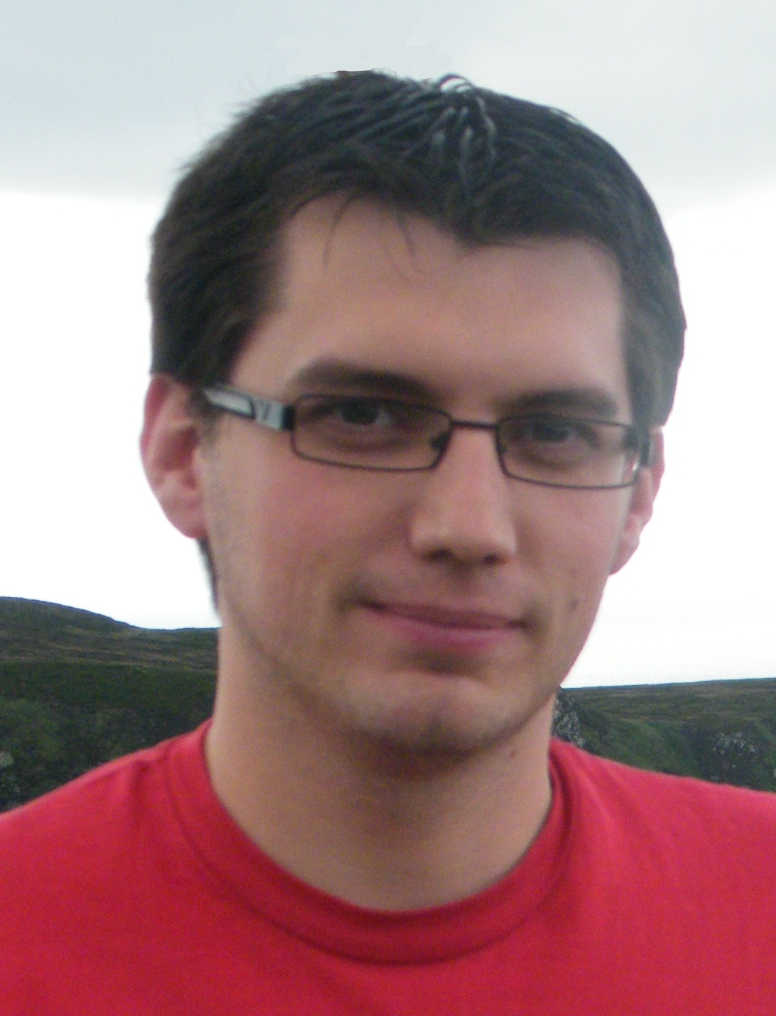
\includegraphics[width=1in,height=1.25in,clip,keepaspectratio]{photos/perez.jpg}}]
{Diego Perez}
is currently pursuing a Ph.D. in Artificial Intelligence applied to games at the University of Essex, Colchester. He has published in the domain of Game AI, participated in several Game AI competitions and organized the Physical Travelling Salesman Problem competitions, held in IEEE conferences. He also has programming experience in the videogames industry with titles published for game consoles and PC.
\end{IEEEbiography}


\begin{IEEEbiography}[{
\includegraphics[width=1in,height=1.25in,clip,keepaspectratio]{photos/sanaz.jpg}}]
{Sanaz Mostaghim}
is a professor of computer science at the Otto von Guericke University Magdeburg, Germany. Her current research interests are in the field of evolutionary computation, particularly in the areas of evolutionary multi-objective optimization, swarm intelligence and their applications in science and industry. She is an active IEEE member and is serving as an associate editor for IEEE Transactions on Evolutionary Computation and IEEE Transactions on Cybernetics.
\end{IEEEbiography}

\begin{IEEEbiography}[{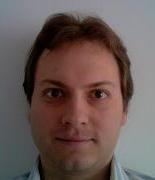
\includegraphics[width=1in,height=1.25in,clip,keepaspectratio]{./photos/spyro.jpg}}]{Spyridon Samothrakis}
 is currently pursuing a PhD in Computational Intelligence and Games at the University of Essex. His interests include game theory, computational neuroscience, evolutionary algorithms and consciousness. 
\end{IEEEbiography}

\begin{IEEEbiography}[{
\includegraphics[width=1in,height=1.25in,clip,keepaspectratio]{photos/lucas.png}}]{Simon Lucas}
(SMIEEE) is a professor of Computer Science at the University of Essex (UK) where he leads the Game Intelligence Group. His main research interests are games, evolutionary computation, and machine learning, and he has published widely in these fields with over 160 peer-reviewed papers. He is the inventor of the scanning n-tuple classifier, and is the founding Editor-in-Chief of the IEEE Transactions on Computational Intelligence and AI in Games.
\end{IEEEbiography}

% You can push biographies down or up by placing
% a \vfill before or after them. The appropriate
% use of \vfill depends on what kind of text is
% on the last page and whether or not the columns
% are being equalized.

%\vfill

% Can be used to pull up biographies so that the bottom of the last one
% is flush with the other column.
%\enlargethispage{-5in}



% that's all folks
\end{document}
